\setlength\parindent{1.25cm}
\pagestyle{plain}
\pagenumbering{arabic}
\setcounter{page}{2}

\refsection

%\clearpage
%\thispagestyle{empty}

%\vfill

%\begin{center}
%[Место для распечатки отчета Антиплагиата]
%\end{center}

%\newpage
%\thispagestyle{empty}

%\vfill

%\begin{center}
%[Место для распечатки отчета Антиплагиата]
%\end{center}

\clearpage

\chapter*{Реферат}
\thispagestyle{plain}

Общий объем основного текста, без учета приложений 38
\pageref{end_of_main_text} страниц, с учетом приложений 44
\pageref{end_of_document}. Количество использованных источников 15.
Количество приложений 1.

%Ключевые слова: 
\noindent \uppercase{микросервисы, golang, распределенные транзакции, postgresql, redpabda}

Целью данной работы является Разработка серверного компонента клиент-серверной
программной системы диагностики щитовидной железы по
ультразвуковым снимкам

В первой главе проводится обзор и анализ предметно области и инстсрументов

Во второй главе описываются использованные и разработанные модели системы и модулей. 

В третьей главе приводится результаты проектирования по разработанным моделям.

%%% Local Variables:
%%% TeX-engine: xetex
%%% eval: (setq-local TeX-master (concat "../" (seq-find (-cut string-match ".*-3-pz\.tex$" <>) (directory-files ".."))))
%%% End:


\clearpage

\tableofcontents{}

\clearpage

\chapter*{Введение}
\label{sec:afterwords}
\addcontentsline{toc}{chapter}{Введение}

Экспертиза щитовидной железы узла является очень сложной и сложной задачей и требует высококвалифицированных медицинских работников. Специальная система классификации EU-TIRADS используется для определения типа узла, основанного на различных особенностях узла, таких как размер, форма и источник эха. Тем не менее, ручная классификация узлов в соответствии с системой EU-TIRADS скучна и может привести к ошибкам.


Из-за широкого использования методов глубокого обучения в различных областях жизни эти методы также используются для решения проблем диагностических эндокринных заболеваний. Чтобы эффективно использовать эти методы в ежедневной работе работников здравоохранения, проводящих эндокринные исследования, необходимо разработать серверные приложения для интуитивного взаимодействия между медицинским персоналом и технологиями искусственного интеллекта.


Целью работы является разработка серверного приложения для упрощения классификации заболеваний в соответствии с EU-TIRADS. Чтобы достичь этой цели, вам необходимо будет разработать архитектуру для вашего приложения для вашего сервера или финансировать существующие, предоставить приложения на единой цифровой платформе российской федерации «ГосТЕХ» и предоставить приложения для измерения скорости обработки и количества запросов, выполняемых одновременно.


Аналогичные технологии уже были реализованы в виде дополнительного программного обеспечения, интегрированного в ультразвуковую диагностику или прикладное программное обеспечение. Однако на данный момент такая технология не представлена ​​на российском рынке. Следовательно, разработка серверных приложений для упрощения классификации заболеваний в EU-TIRADS является важным шагом в разработке эндокринной диагностики.

%%% Local Variables:
%%% TeX-engine: xetex
%%% eval: (setq-local TeX-master (concat "../" (seq-find (-cut string-match ".*-3-pz\.tex$" <>) (directory-files ".."))))
%%% End:


\clearpage

\chapter{Анализ подходов к разработке серверных приложений ИИ ассистентов}
\label{chapter1}

\section{Анализ применения ИИ ассистентов в медицине}

\subsection{Анализ основных областей применения ИИ ассистентов}
Государственное направление по улучшению всех жизненных сфер путем оцифровки, приводит к многочисленным инновациям и крупномасштабным ИТ-проектам. Реализация информационных технологий происходит в области здравоохранения это ключевой показатель уровня жизни страны.\\
Первоначально цифровизация медицины была предназначена для повышения диагностической эффективности и сокращения времени, необходимого для предоставления медицинских услуг. Рутина и сложные задачи передаются на производительность устройства и выполняются с использованием различных технических достижений. С этой целью были созданы многие системы и платформы, которые сокращают время для реализации стандартных диагностических процессов. В этом списке системы с искусственным интеллектом (ИИ) могут быть важны для замены ручной работы интеллектуальными навыками из различных отраслей. Искусственный интеллект - это область науки и техники, которая позволяет компьютерам и программам выполнять интеллектуальные задачи. У него есть возможность выполнять различные задачи, учиться при их использовании и адаптироваться к новым задачам и контекстам. Кроме того, ИИ может выступать в качестве дополнительной аналитической перспективы, позволяя упростить многие процессы с помощью анализа данных и вопросов поиска схемы.\\
Искусственный интеллект может изменить систему здравоохранения, автоматизируя многие из ее аспектов, позволяя сотрудникам сосредоточиться на основных задачах, связанных с уходом и лечением пациентов. Системы здравоохранения на основе искусственного интеллекта являются отличительной скоростью, дополненными простым использованием и снижением затрат, что делает их неотъемлемой частью разработки.\\
Сфера здоровья, в которой активно используется искусственный интеллект, может быть разделена на четыре основных частей.

\begin{itemize}
    \item используется графическая информация (анализ результатов радиационной диагностики).
    \item принятие и диагноз на основе различных метаданных.
    \item Дистанционные консультации и обеспечение контроля здоровья пациентов.
    \item Исследование лекарств, создание и реализация.
\end{itemize}

\subsection{Обзор существующих систем поддержки принятия врачебных решений с применением искусственного интеллекта}
В России значительное число медицинских компаний и стартапов также используют искусственный интеллект для поддержки медицинских решений. Основными областями работы являются анализ исследований на флуоресцентных (FLG), X-Ray -изображениях (RG) и компьютерной томографии (КТ).\\
Крупнейшие ИИ медицинские системы:\\
\begin{itemize}
    \item MDDC создается для поддержки медицинских решений в соответствии с первоначальным диагнозом, инструментами и лабораториями. Система интегрирована в различные системы данных и источники данных и использование технологий искусственного интеллекта для обработки и анализа данных о здоровье.
    \item Celsus - это система поддержки медицинских решений, основанных на технологиях искусственного интеллекта, позволяя вам анализировать цифровые медицинские изображения, обнаруживать объекты и автоматически формировать результаты. Основными областями разработки являются анализ изображений X-RAY и флуорографии, анализ КТ и легких.
    \item «ФтизисБиоМед», продукты и услуги широко используются в практической медицине, чтобы снизить неправильный диагноз и обеспечить раннюю диагностику на ранних стадиях заболевания. Среди наиболее важных событий в компании можно выделить услуги для анализа медицинских изображений (флурограмма и X-Rays) на основе ИИ.
\end{itemize}
Основываясь на анализе лидеров в области исследований искусственного интеллекта в области медицины, мы можем сделать вывод, что ультразвуковой анализ щитовидной железы является одной из наиболее актуальной задач. Выбор области исследований и скачок в финансировании проектов медицинских технологий произошел в 2020 году, объясняющий эпидемиологическую ситуацию с Covid-19. Самым важным решением, принятым в то время, был постановление правительства о оцифровке системы здравоохранения и создании различных государственных платформ здравоохранения поэтому решение создать полную систему для диагностики гормональных заболеваний в соответствии с изображением узи снимков является наиболее перспективным способом достижения цели на работе.\\
Кроме того, основные направления задач выполняются с помощью систем, которые можно различить это обнаружение патологии на основании графических результатов клинических исследований и предварительной диагностики. Этот выбор обусловлен сложностью диагностического процесса и необходимостью высокой подготовки для экспертов.\\


\section{Анализ основных архитектур для построения серверных приложений}

Традиционная архитектура на основе клиент-серверной модели является одной из наиболее распространенных архитектур для создания серверных приложений. Эта модель предполагает разделение приложения на две составляющие - клиентскую и серверную. Клиентская составляющая отвечает за интерфейс взаимодействия с пользователем, а серверная - за обработку запросов и предоставление данных.
Основным преимуществом клиент-серверной модели является возможность создания распределенной архитектуры, которая позволяет создавать приложения с большими объемами данных или с большим количеством пользователей. Также этот подход позволяет легко масштабировать и обновлять серверное приложение без влияния на клиентскую составляющую.
Одним из недостатков клиент-серверной модели является ее зависимость от сети. Отказ сети или недоступность сервера может привести к невозможности доступа к приложению. Еще одним недостатком является необходимость настройки и поддержки серверной инфраструктуры, что может требовать отдельных затрат и увеличить стоимость разработки и поддержки серверного приложения.
Для реализации клиент-серверной модели на практике используются различные технологии и инструменты, как проприетарные, так и открытые. Например, для создания серверных приложений могут использоваться языки программирования, такие как Golang, Java, Python, Ruby, PHP, а для создания клиентских приложений - HTML, CSS, JavaScript.
Существует также множество фреймворков, библиотек и инструментов, которые предназначены для упрощения разработки серверных приложений на основе клиент-серверной модели. Например, Node.js является популярным фреймворком для создания серверных приложений на JavaScript, а Django и Flask - для Python.
Также используются такие средства, как базы данных, предназначенные для хранения данных приложения, или сервисы и инструменты для автоматизации и управления развертыванием и масштабированием серверных приложений. Кроме того, существуют такие платформы, как Яндекс Облако и Selectel, которые предоставляют в облаке готовые инструменты для создания и развертывания серверных приложений на основе клиент-серверной модели.

\subsection{Микросервисная архитектура}

Микросервисная архитектура является относительно новым подходом к разработке серверных приложений. Она характеризуется модульностью, то есть каждый модуль является отдельным сервисом, который может быть развернут и масштабирован отдельно от других модулей. Микросервисная архитектура рассматривает приложение как совокупность небольших сервисов, которые представляют отдельные функции приложения. Каждый сервис обычно работает независимо от других сервисов, используя API для обмена данными между другими сервисами.
Основное преимущество микросервисной архитектуры заключается в ее модульности\cite{newman2019monolith}. Это дает возможность быстро отвечать на изменения требований и легко масштабировать приложение по мере необходимости. Другим преимуществом микросервисной архитектуры является возможность использования различных технологий и языков программирования для различных сервисов. Это позволяет использовать наилучшее решение для каждой отдельной задачи. Микросервисная архитектура может быть также более устойчивой и надежной, поскольку имеется возможность аварийного отключения отдельных сервисов, позволяя уменьшить влияние отказа других компонентов на работу приложения в целом.
Существует несколько типов микросервисных архитектур, которые различаются по тому, как организованы и взаимодействуют между собой микросервисы. К одному из распространенных типов микросервисных архитектур относится оркестрованная архитектура [8] – это такая архитектура, в которой существует централизованный компонент или слой, называемый оркестратором, который координирует действия и взаимодействие других микросервисов в системе. Оркестратор отвечает за управление жизненным циклом запросов от клиентов, контроль последовательности выполнения операций и обработку бизнес-логики интеграции между сервисами. 
Ещё одним из распространённых типов микросервисных архитектур является event-driven архитектура – архитектура, в которой микросервисы взаимодействуют через отправку и прием событий. Каждый сервис может публиковать события, на которые другие сервисы могут, соответственно, подписываться и реагировать. К её преимуществам относятся: гибкость (компоненты могут быть легко добавлены или удалены без влияния на другие части системы), масштабируемость (каждый компонент может масштабироваться независимо для обеспечения высокой производительности), отказоустойчивость (отказ одного компонента не блокирует работу всей системы). Однако тут возникает сложность в обеспечении согласованности данных между различными сервисами, управлении событиями и обработке ошибок.
Также стоит упомянуть про подход API Gateway – данный тип архитектуры использует централизованный шлюз, который является единой точкой входа для всех запросов клиентов к микросервисам или другим системам. Шлюз может выполнять несколько функций, к которым относятся: аутентификация, авторизация, маршрутизация запросов, преобразование протоколов и форматов данных, кеширование, балансировка трафика и другие. Данный подход позволяет сделать архитектуру приложения более гибкой, безопасной и легкой в управлении, а также позволяет централизованно управлять всеми взаимодействиями клиентов с микросервисами, упрощая развертывание и поддержку системы.

Микросервисная архитектура предусматривает разбиение приложения на небольшие независимые сервисы, каждый из которых выполняет строго определённые задачи. Эти сервисы взаимодействуют через сети с использованием API или брокеров сообщений.

\textbf{Преимущества микросервисной архитектуры}:
\begin{itemize}
    \item \textbf{Гибкость масштабирования:} отдельные сервисы масштабируются независимо, что оптимизирует использование ресурсов.
    \item \textbf{Свобода выбора технологий:} команды могут использовать разные языки программирования и инструменты для реализации отдельных сервисов.
    \item \textbf{Лучшая управляемость:} изолированные сервисы упрощают внесение изменений и поддержку.
    \item \textbf{Повышенная устойчивость:} сбой одного сервиса не влияет на работу других\cite{richards2015patterns}.
    \item \textbf{Параллельная разработка:} команды могут работать над разными сервисами одновременно.
\end{itemize}

\textbf{Недостатки микросервисной архитектуры}:
\begin{itemize}
    \item \textbf{Сложность проектирования:} требует тщательного планирования взаимодействия между сервисами.
    \item \textbf{Проблемы с согласованностью данных:} переход к eventual consistency добавляет сложности.
    \item \textbf{Высокие инфраструктурные затраты:} управление множеством сервисов требует дополнительных инструментов, таких как Kubernetes.
    \item \textbf{Увеличение задержек:} сетевое взаимодействие между сервисами медленнее, чем вызовы в памяти.
    \item \textbf{Сложности диагностики:} распределённый характер системы затрудняет выявление и исправление ошибок.
\end{itemize}

\subsection{Монолитная архитектура}

Монолитная архитектура представляет собой подход, при котором всё приложение разрабатывается как единый, неделимый блок\cite{vernon2022strategic}. В нём объединены пользовательский интерфейс, бизнес-логика и уровень работы с данными. Такой подход исторически был основным в разработке ПО.

\textbf{Преимущества монолитной архитектуры}:
\begin{itemize}
    \item \textbf{Простота разработки:} начальный этап разработки требует меньше усилий на планирование структуры.
    \item \textbf{Единая кодовая база:} централизованное хранение и управление кодом упрощает процесс разработки и интеграции изменений.
    \item \textbf{Простая инфраструктура:} одно монолитное приложение, не требует дополнитнельных расходов на инфраструктуру.
    \item \textbf{Высокая производительность:} отсутствие сетевого взаимодействия между компонентами ускоряет их взаимодействие.
    \item \textbf{Поддержка транзакционности:} встроенные механизмы работы с транзакциями позволяют обеспечить согласованность данных.
\end{itemize}

\textbf{Недостатки монолитной архитектуры}:
\begin{itemize}
    \item \textbf{Сложность масштабирования:} увеличение нагрузки требует масштабирования всего приложения, даже если это касается лишь одного его компонента.
    \item \textbf{Ограничения технологического выбора:} единая технологическая платформа ограничивает возможности внедрения новых инструментов.
    \item \textbf{Рост сложности кода:} по мере увеличения объёма функциональности поддержка системы становится сложнее.\cite{al-debagy2019review}
    \item \textbf{Долгое развертывание:} внесение малейших изменений требует пересборки и перезапуска приложения.
    \item \textbf{Уязвимость к сбоям:} сбой в одном компоненте приводит к отказу всей системы.
\end{itemize}


\subsection{Сравнение монолитной и микросервисной архитектур}

Для более наглядного понимания различий между монолитной и микросервисной архитектурами представим их основные аспекты в таблице\cite{dragoni2017scale}:

\begin{table}[H]
\centering
\begin{tabular}{|l|l|l|}
\hline
\textbf{Аспект}                & \textbf{Монолит}       & \textbf{Микросервисы}   \\ \hline
Сложность разработки           & Низкая                                 & Высокая                                \\ \hline
Масштабируемость               & Ограниченная                           & Гибкая                                 \\ \hline
Устойчивость к сбоям           & Низкая                                 & Высокая                                \\ \hline
Технологический выбор          & Ограниченный                           & Гибкий                                 \\ \hline
Развертывание                  & Простое                                & Сложное                                \\ \hline
Поддержка транзакционности     & Простая                                & Сложная                                \\ \hline
Задержки взаимодействия        & Минимальные                            & Увеличенные                            \\ \hline
Затраты на инфраструктуру      & Низкие                                 & Высокие                                \\ \hline
\end{tabular}
\caption{Сравнение монолитной и микросервисной архитектур}
\end{table}

\textbf{Выводы:} Монолитная архитектура лучше подходит для проектов с ограниченным функционалом и небольшими командами, где важны простота и быстрота разработки. Микросервисы же оправданы в сложных, масштабируемых системах с распределёнными командами и высокими требованиями к отказоустойчивости.\cite{shadija2017understanding}













\section{Анализ и сравнение паттернов проектирования модулей системы}

Связанность (англ. Coupling) и согласованность (англ. Cohesion) являются фундаментальными концепциями в области разработки программного обеспечения, которые оказывают значительное влияние на читаемость, поддержку, тестируемость и переиспользование кода\cite{vernon2013implementing}. В данной работе исследуются эти понятия, их виды, а также взаимосвязь между ними с целью формирования рекомендаций по их применению для повышения эффективности разработки.

\subsection*{Связанность (Coupling)}

Связанность характеризует степень зависимости одного программного модуля от других\cite{fowler1999patterns}. Чем выше уровень связанности, тем сильнее изменения в одном модуле отражаются на других. Стремление к низкой связанности (low coupling) является ключевым принципом проектирования, позволяющим минимизировать количество зависимостей между модулями и повысить их автономность.

Существует несколько типов связанности, классифицируемых по степени их зависимости:

\begin{itemize}
    \item \textbf{Content coupling} (содержательная связанность): возникает, когда один модуль полагается на внутреннюю реализацию другого модуля, например, доступ к его локальным данным. Изменения в одном модуле требуют изменений в другом.
    \item \textbf{Common coupling} (общая связанность): модули используют общие данные, например, глобальные переменные. Изменение этих данных затрагивает все модули, которые с ними работают.
    \item \textbf{External coupling} (внешняя связанность): несколько модулей зависят от общего внешнего ресурса, такого как сервис или API. Изменения в этом ресурсе могут привести к некорректной работе модулей.
    \item \textbf{Control coupling} (управляющая связанность): один модуль управляет поведением другого через передачу управляющих сигналов, например, флагов, изменяющих поведение функций.
    \item \textbf{Stamp coupling} (штампованная связанность): модули обмениваются сложными структурами данных, однако используют лишь их часть. Это может приводить к побочным эффектам из-за неполной или изменяемой информации.
    \item \textbf{Data coupling} (связанность по данным): наименее инвазивный тип, при котором модули взаимодействуют исключительно через передачу конкретных данных. Такой подход минимизирует взаимозависимость.
\end{itemize}

\subsection*{Согласованность (Cohesion)}

Согласованность характеризует степень внутренней связанности функциональных элементов модуля\cite{meyer1997object}. Высокая согласованность подразумевает, что все компоненты модуля ориентированы на выполнение одной конкретной задачи или функции, что улучшает читаемость и управляемость кода.

Типы согласованности включают:

\begin{itemize}
    \item \textbf{Functional cohesion} (функциональная согласованность): модуль объединяет весь необходимый функционал для выполнения одной задачи.
    \item \textbf{Sequential cohesion} (последовательная согласованность): результаты одной функции используются в качестве входных данных для другой.
    \item \textbf{Communication cohesion} (коммуникационная согласованность): все элементы модуля работают с одними и теми же данными.
    \item \textbf{Procedural cohesion} (процедурная согласованность): элементы модуля выполняются в определенной последовательности, необходимой для достижения результата.
    \item \textbf{Temporal cohesion} (временная согласованность): функции модуля сгруппированы на основе их выполнения в определенный момент времени (например, при обработке ошибок).
    \item \textbf{Logical cohesion} (логическая согласованность): элементы модуля объединены логически общей функцией, но могут отличаться по своей природе (например, обработка различных типов ввода).
    \item \textbf{Coincidental cohesion} (случайная согласованность): элементы модуля не связаны логически, что делает модуль хаотичным и сложным для понимания.
\end{itemize}

\subsection*{Взаимосвязь между Coupling и Cohesion}

Связанность и согласованность находятся в сложной взаимозависимости\cite{bon2020adaptive}. Уменьшение связанности обычно способствует увеличению согласованности и наоборот. Например, избыточная согласованность может привести к росту зависимости между модулями, что увеличивает связанность. Таким образом, ключевым аспектом является нахождение оптимального баланса, который обеспечит поддержку высокого уровня согласованности при минимально возможной связанности.

Применение принципов низкой связанности и высокой согласованности позволяет создавать поддерживаемые, масштабируемые и понятные программные системы. Их использование способствует не только повышению качества кода, но и ускорению разработки, что особенно важно в современных условиях высокой конкуренции и быстрого изменения требований.





\subsection{Луковая архитектура}
\textbf{Луковая архитектура} была предложена Джеффри Палермо в 2008 году как расширение гексагональной архитектуры\cite{palermo2008onion}. Её цель — облегчить поддержку приложений за счёт разделения аспектов и строгих правил взаимодействия слоёв.

\subsubsection{Основная идея}
Луковая архитектура предполагает многослойную организацию системы, где каждый слой зависит только от внутреннего слоя. Центральным слоем всегда является независимый слой, который представляет собой сердцевину архитектуры. Остальные слои располагаются вокруг него, создавая структуру, похожую на лук.

\textbf{Ключевые принципы:}
\begin{itemize}
    \item Приложение строится вокруг независимой объектной модели.
    \item Внутренние слои определяют интерфейсы, внешние — реализуют их.
    \item Зависимости направлены к центру.
    \item Код предметной области изолирован от инфраструктуры.
\end{itemize}

\subsubsection{Слои}
\textbf{Domain Model:} содержит основные сущности и поведение предметной области, например, валидацию данных.

\textbf{Domain Services:} реализует бизнес-логику, которая не связана с конкретными сущностями, например, расчёт стоимости заказа.

\textbf{Application Services:} оркестрирует бизнес-логику, например, обработку запроса на создание заказа.

\textbf{Infrastructure:} реализует интерфейсы и адаптеры для работы с базами данных, внешними API и другими ресурсами.

\subsubsection{Преимущества}
\begin{itemize}
    \item Независимость предметной области от инфраструктуры.
    \item Гибкость замены внешних слоёв.
    \item Высокая тестируемость.
\end{itemize}

\subsubsection{Недостатки}
\begin{itemize}
    \item Сложность обучения.
    \item Необходимость создания множества интерфейсов.
\end{itemize}

\subsection{Hexagonal Architecture}
\textbf{Hexagonal Architecture} (также известная как Ports and Adapters) была предложена Alistair Cockburn\cite{cockburn2005hexagonal}. Её цель — устранить зависимость бизнес-логики от внешних систем и сделать приложение более гибким и тестируемым.

\subsubsection{Основная идея}
Hexagonal Architecture представляет приложение в виде шестиугольника\cite{garg2022demystifying}, где каждая сторона представляет интерфейс (порт) для взаимодействия с внешними системами (адаптерами). Центр архитектуры — это бизнес-логика, изолированная от деталей реализации.

\textbf{Ключевые принципы:}
\begin{itemize}
    \item Бизнес-логика полностью изолирована от инфраструктуры.
    \item Взаимодействие с внешним миром происходит через порты и адаптеры.
    \item Внешние системы подключаются через адаптеры, соответствующие определённым портам.
\end{itemize}

\subsubsection{Слои}
\textbf{Core (Business Logic):} центральная часть архитектуры, содержащая доменные сущности и бизнес-правила.

\textbf{Ports:} интерфейсы, через которые осуществляется взаимодействие между Core и внешними системами.

\textbf{Adapters:} реализация портов для подключения конкретных технологий, таких как базы данных, веб-сервисы и т.д.

\subsubsection{Преимущества}
\begin{itemize}
    \item Гибкость: легко заменять внешние системы, не затрагивая бизнес-логику.
    \item Тестируемость: изолированная бизнес-логика упрощает написание модульных тестов.
    \item Чёткое разделение обязанностей.
\end{itemize}

\subsubsection{Недостатки}
\begin{itemize}
    \item Сложность проектирования и реализации.
    \item Дополнительные накладные расходы на создание портов и адаптеров.
\end{itemize}

\subsection{Чистая архитектура}
\textbf{Чистая архитектура}, предложенная Робертом Мартином, основывается на идеях Onion и Hexagonal архитектур\cite{martin2017clean}

\subsubsection{Базовые принципы}
\begin{itemize}
    \item Использование принципов SOLID.
    \item Разделение системы на слои.
    \item Независимость бизнес-логики от инфраструктуры.
    \item Тестируемость бизнес-логики без внешних зависимостей.
\end{itemize}

\subsubsection{Слои}
\textbf{Domain:} содержит общие бизнес-правила, структуры и интерфейсы.

\textbf{Application:} реализует конкретные сценарии использования, например, обработку запросов.

\textbf{Presentation:} отвечает за взаимодействие с пользователем через REST API, CLI и т.д.

\textbf{Infrastructure:} содержит детали реализации, такие как доступ к базе данных или внешние сервисы.

\subsubsection{Пересечение границ}
В чистой архитектуре зависимости направлены внутрь\cite{hombergs2020dirty}. Внешние слои реализуют интерфейсы, определённые внутренними слоями. Это достигается за счёт принципа инверсии зависимостей (DIP).

\subsubsection{Преимущества}
\begin{itemize}
    \item Независимость от фреймворков и инфраструктуры.
    \item Простота тестирования.
    \item Переносимость и возможность разделения на микросервисы.
\end{itemize}

\subsubsection{Недостатки}
\begin{itemize}
    \item Требуется строгое разделение бизнес-правил.
    \item Возможность излишнего усложнения структуры.
\end{itemize}


\textbf{Вывод}


\textbf{Чистая архитектура} представляет собой эволюцию луковой и гексагональной архитектур, сохраняя их принципы, но делая больший акцент на SOLID и изоляции бизнес-логики. Она подходит для сложных систем, требующих высокой гибкости и тестируемости, но может быть избыточной для небольших приложений.


% Это обзорно-аналитическая глава, в которой требуется отразить:

% \begin{itemize}
% 	\item результат изучения различных существующих методов решения задач в рамках проблематики УИРа/диплома (иногда даже в смежных областях), это обзорный аспект, который пишется, в основном, на основе имеющейся литературы или/и программного обеспечения;
% 	\item сравнение (с какой-либо определенной целью) этих методов и средств.
% \end{itemize}

% Приведенные ниже названия пунктов являются очень примерными, их состав и структура сильно зависят от специфики конкретной работы.




% %Большие отсупы --- это хорошо. Облегчает чтение длинных <<простыней>> текста
% \section{Общий анализ проблематики \dots}

% \begin{annotation}
% В случае РСПЗ, так оформляется аннотация к разделу. Такая же аннотация, только более общая, должна быть для главы. После аннотации может следовать рабочая или финальная версия текста соответствующего раздела. В случае ПЗ, таких аннотаций быть не должно.
% \end{annotation}

% \dots

% Результаты анализа полезно оформлять в виде таблиц (см. табл. \ref{tbl:cmp-1}).

% \begin{table}%
% \caption{Результаты сравнения нескольких программных систем}\label{tbl:cmp-1}
% \centering
% \begin{tabular}{|l|l|c|c|c|c|}

% \hline

% \textnumero & Название системы & Показатель 1 & Показатель 2 & Показатель 3 & Показатель 4 \\

% \hline

% \end{tabular}
% \end{table}


% \section{Анализ особенностей \dots}

% Сначала приведем пример более сложной таблицы (см. табл. \ref{tbl:cmp-adv} и 
% \ref{tbl:cmp-2}).

% \begin{table}%
% \caption{Таблица с длинным, многострочным названием, чтобы показать, как форматируется такой заголовок}
% \label{tbl:cmp-adv}
% \centering
% \begin{tabular}{|l|l|c|c|c|c|}

% \hline

% \textnumero & Название системы & Показатель 1 & Показатель 2 & Показатель 3 & Показатель 4 \\

% \hline

% \end{tabular}
% \label{tbl:cmp-2}
% \end{table}


% А теперь, продемонстрируем, как должна выглядеть иллюстрация (см. рис. \ref{pic:lambda-cube}).

% \begin{figure}[t]%
% \begin{center}
% \includegraphics[width=.5\columnwidth]{./img/lambda-cube.png}%
% \end{center}
% \caption{Ламбда-куб Барендрегта}%
% \label{pic:lambda-cube}%
% \end{figure}

% А теперь, продемонстрируем, как должна выглядеть иллюстрация с длинной подрисуночной подписью (см. рис. \ref{pic:lambda-cube-long-caption}).

% \begin{figure}[t]%
% 	\begin{center}
% 		\includegraphics[width=.5\columnwidth]{./img/lambda-cube.png}%
% 	\end{center}
% 	\caption{Ламбда-куб Барендрегта, иллюстрирующий многообразие систем типизации с точки зрения четырех базовых видов зависимостей между типами и объектами: термов от термов, термов от типов, типов от типов и типов от термов.}%
% 	\label{pic:lambda-cube-long-caption}%
% \end{figure}

% \subsection{Ссылки на литературу}

% В этой версии шаблона используется BibLaTeX, основанный на biber и BibTeX.
% Поэтому для оформления списка литературы используются два файла:
% \texttt{thesis-bibl.tex} и \texttt{biblio.bib}. Использование BibTex дает ряд
% преимуществ. Не нужно заботиться о порядке сортировки, это делается
% автоматически; не нужно заботиться, на какие элементы библиографии есть ссылки
% --- печатаются только использованные в тексте элементы. Кроме того, многие
% курсовые проекты выполняются на протяжении ряда лет. С BibTex проще собирать
% список литературы и управлять им.

% На все элементы списка литературы должны быть ссылки из текста. При
% использовании команды \texttt{\textbackslash{}cite} это происходит
% автоматически. Отсутствиессылок на литературу из текста допускается в РСПЗ,
% т.~е. в РСПЗ список литературы скорее имеет смысл списка подобранной литературы
% по теме или библиографии. Для того, чтобы в списке литературы отобразились
% источники, на которые отсутствуют ссылки в тексте, следует использовать команду
% \texttt{\textbackslash{}nocite}. К примеру, \texttt{\textbackslash{}nocite\{*\}}
% выводит в список литературы все содержимое подключенных BibTeX файлов, вставляя
% невидимые ссылки на них.

% \section{Сравнительный анализ алгоритмов \dots}

% \dots





% \section{Сравнительный анализ программных средств \dots}

% \dots




\section{Выводы}

\begin{enumerate}
    \item Разобраны основные методы применения ИИ в медицине. Особенности применения ИИ ассистентов в работе врача, основные аналоги систем ИИ ассистентов представленных на рынке.
	\item Выполнен анализ архитектурных стилей построения систем, с учетом требований к динамической расширяемости отдельных модулей системы, выбрана микросервисная архитектура с применением API Gateway.
	\item Проанализированы основные архитектурные паттерны построения приложений. Clean Architecture за счет преобраладания SOLID, разбиения на слои и преимуществ Dependency inversion выбрана как основа написания микросервисов.
\end{enumerate}

\section{Постановка цели и задач ВКР}

Целью данной ВКР является разработка системы серверного приложения комплексной системы «Интеллектуальный ассистент врача УЗИ».


Задачи на ВКР:
\begin{enumerate}
    \item Разграничение функционала серверного приложения на доменные области.
    \item Проектирование системы Интеллектуальный ассистент врача УЗИ, с учетом разграничения на доменные области.
    \item Реализация микросервисов в соответствии с принципами Clean Architecture.
	\item Тестирование разработанной системы и ее производительности. Устранение недостатков при наличии.
\end{enumerate}

% Разграничение функционала серверного приложения на изолированные предметные области области.
% Проектирование системы Интеллектуальный ассистент врача УЗИ, с учетом разграничения на предметные области.
% Реализация микросервисов в соответствии с принципами Clean Architecture.
% Тестирование разработанной системы и устранение недостатков при наличии.



%%% Local Variables:
%%% TeX-engine: xetex
%%% eval: (setq-local TeX-master (concat "../" (seq-find (-cut string-match ".*-3-pz\.tex$" <>) (directory-files ".."))))
%%% End:


\clearpage

 \chapter{Теоретическая часть}

\section{Модель микросервиса}

К каждому микросервису выделяются общие функциональные требования:
\begin{itemize}
  \item При необходимости выполнять CRUD операции с базой данных
  \item При необходимости писать сообщения в логброкер сообщений
  \item При необходимости читать сообщения из логброкера сообщений
\end{itemize}

К каждому микросервису выделяются общие нефункциональные требования:
\begin{itemize}
  \item Соответствовать чистой архитектуре
  \item Иметь высокий cohesion и низкие coupling
\end{itemize}


Исходя из этих требований, типовая архитектура нашего сервиса будет соответствовать приведенной.

\begin{figure}[H]%
	\begin{center}
		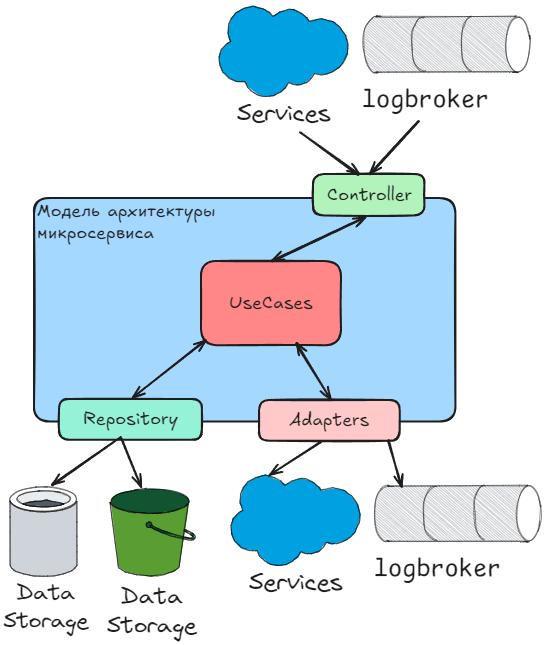
\includegraphics[width=.5\columnwidth]{./img/tipovoy_micric.png}%
	\end{center}
	\caption{Модель типового микросервиса}%
	\label{pic:tipovoy_micric}%
\end{figure}

\section{Модели модулей системы}
\subsection{Модель сервиса аутентификации}

Микросервис аутентификации осуществляет регистрацию новых пользователей, и обновление токенов у уже существующих.
Для сущесвующих пользователей он выдает новую пару JWT tokens(access token + refresh token) по refresh token или логину
и паролю.

Функциональные требования к сервису аутентификации:
\begin{itemize}
  \item Возможность регистрировать новых пользователей в сервисе
  \item Подписывать JWT ключи для авторизации
  \item Обменивать логин пароль или refresh JWT ключ на новый resfresh JWT ключ
\end{itemize}

Тогда для соответствия требованиям, модель базы данных:
\begin{figure}[H]%
	\begin{center}
		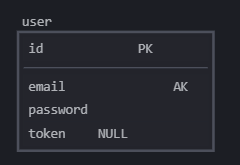
\includegraphics[width=.5\columnwidth]{./img/auth_db_model.png}%
	\end{center}
	\caption{Модель базы данных сервиса аутентификации}%
	\label{pic:auth_db}%
\end{figure}


Для обмена refresh token на новую пару ключей, в токен необходимо зашивать ID пользователя.
В соответствии с требованиями, модель сервиса авторизации:
\begin{figure}[H]%
	\begin{center}
		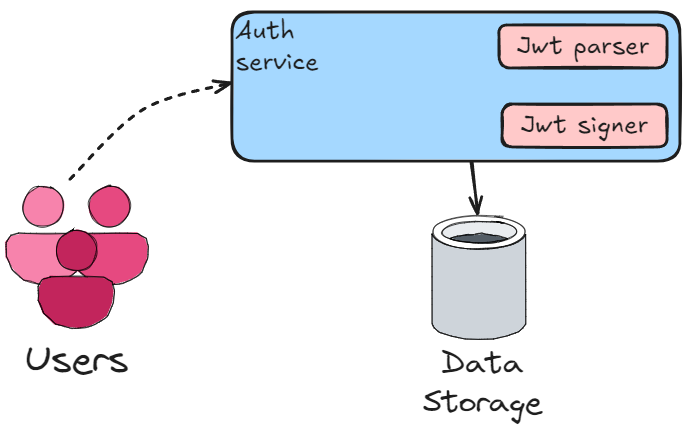
\includegraphics[width=.5\columnwidth]{./img/auth_model.png}%
	\end{center}
	\caption{Модель сервиса аутентификации}%
	\label{pic:auth_model}%
\end{figure}


\subsection{Модель сервиса узи}
Для начала нужно определить вид данных которые должен хранить узи.

Узи представляет из себя последовательный набор кадров, конкретной щитовидной железы. На щитовидной
железе могут быть обнаружены злокачественные образования, называемыми \textbf{узлами}. Узел злокачественного образования
может быть запечатлен на нескольких кадрах, такое отображения узла на конкретном кадре называется \textbf{сегмент}ом,
узлов может быть любое количество. Каждый узел и сегмент в отдельности характеризуется классификационными признаками.
На данный момент имеется 3 классификациооных признака: вероятности принадлежности узлов к классам \textbf{TI-RADS}.
TI-RADS, описывает стадию злокачественного образования, существует 3 стадии: TI-RADS23, TI-RADS4, TI-RADS5.

Функциональные требования к сервису узи:
\begin{itemize}
  \item Принимать единуб композицию кадров узи, разбивать и сохранять ее по кадрам.
  \item После разбиения узи по кадрам, оповещать через брокер сообщений, сервис с ml моделью, о доступности обработки изображения
  \item Предоставлять возможность совершать CRUD операции над узлами, сегментами, узи, ti-rads, images.
  \item Сохранять результат сегментации и классификации нейронной моделью посредством логброкера сообщений.
\end{itemize}


Тогда для соответствия требованиям, модель базы данных:
\begin{figure}[H]%
	\begin{center}
		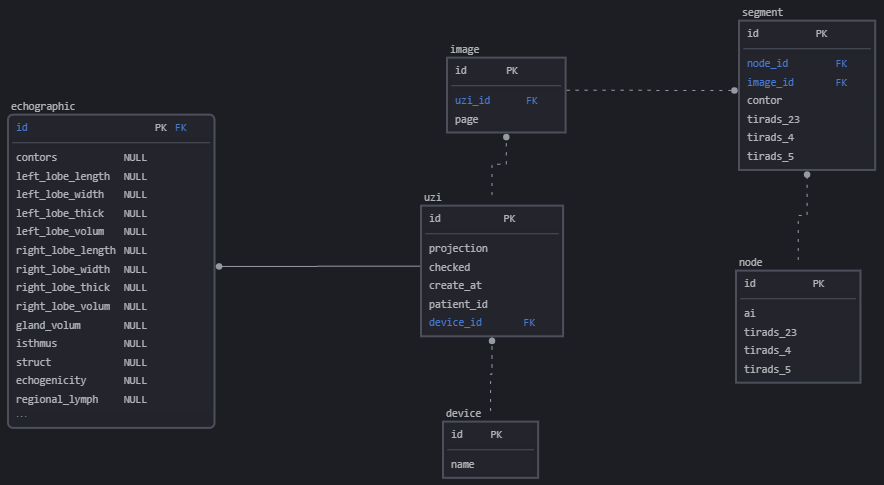
\includegraphics[width=.5\columnwidth]{./img/uzi_db_model.png}%
	\end{center}
	\caption{Модель базы данных сервиса аутентификации}%
	\label{pic:auth_db}%
\end{figure}


В соответствии с требованиями, модель сервиса узи:
\begin{figure}[H]%
	\begin{center}
		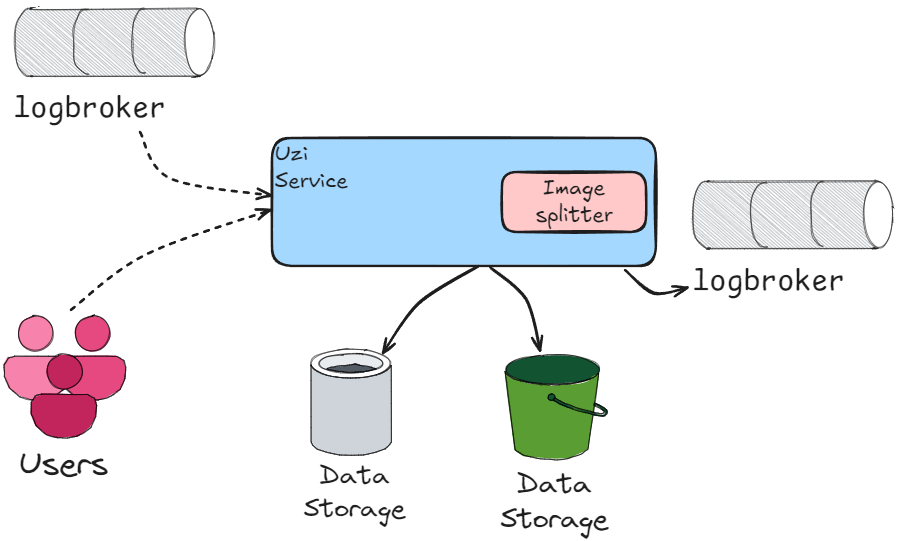
\includegraphics[width=.5\columnwidth]{./img/uzi_model.png}%
	\end{center}
	\caption{Модель сервиса УЗИ}%
	\label{pic:auth_model}%
\end{figure}


\subsection{Модель Gateway API}
Сервис gateway API, является точной входа для всех пользователей системы. Сервис делает запросы в дочерние микросервисы.


Функциональные требования к сервису Gateway API:
\begin{itemize}
  \item Если дочерний микросервис реализует публичный для пользователя контракт взаимодействия, то сервис должен реализовывать доступ к этому контракту для пользователя
  \item Предоставлять пользователю по запросу кадры узи
  \item Запускать пайплайн обработки узи, посредством сообщения в логброкер
\end{itemize}


В соответствии с требованиями, модель сервиса Gateway:
\begin{figure}[H]%
	\begin{center}
		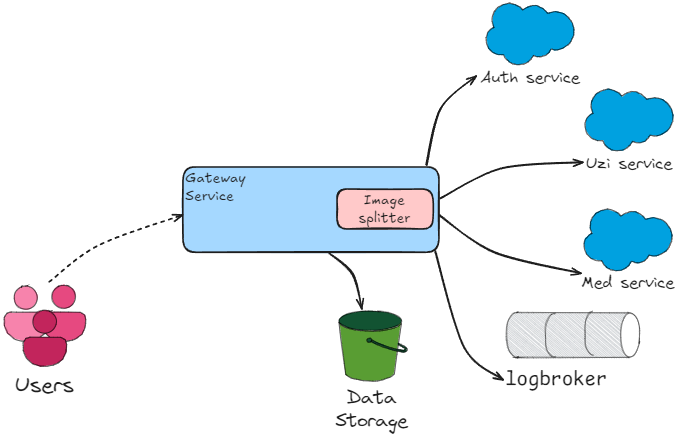
\includegraphics[width=.5\columnwidth]{./img/gateway_model.png}%
	\end{center}
	\caption{Модель сервиса gateway}%
	\label{pic:auth_model}%
\end{figure}

% В этой главе описываются разработанные/модифицированные модели/методы/
% алгоритмы, или/и описывается применение известных стандартных методов. Также, 
% в конце главы обычно приводится общая архитектура программной системы, 
% вытекающая из описанной теории. Приведенные ниже заголовки подразделов так же 
% весьма примерные и сильно зависят от особенностей конкретной работы.

% Формулы и их части необходимо набирать в математическом режиме
% (символ \verb|$|). Во избежание переноса длинных формул между строками их 
% стоит размещать по центру колонки, например,
% \begin{center}
% $S a b c = (\lambda x y z. x z (y z)) a b c = a c (b c)$,
% \end{center}
% \noindent и, если абзац после формулы продолжается, необходимо использовать 
% \verb|\noindent|.

% Для набора правил вывода можно использовать пакет \texttt{mathpartir.sty}. 
% Правила вывода могут быть вынесены в виде рисунка (см. рис. 
% \ref{img:inferrules}).

% \begin{figure}[t]
%   \centering
%     \begin{mathpar}
%       \inferrule{
%         M \to M'
%       }{
%         N M \to N M'
%       } \quad (\mu) \and 
%       \inferrule{
%         M \to M'
%       }{
%         M N \to M' N
%       } \quad (\nu) \and
%       \inferrule{
%         M \to M'
%       }{
%         \lambda x. M \to \lambda x. M'
%       } \quad (\xi)
%     \end{mathpar}
%   \caption{Правила редукции}
%   \label{img:inferrules}
% \end{figure}

% Для оформления определений, теорем, доказательств и т.~п. могут быть 
% использованы соответствующие окружения, например:

% \begin{definition}
% (высказывание)
% Высказыванием называется любое истинное или ложное утверждение.
% \end{definition}


% \section{Модель системы \dots}

% \dots




% \section{Метод решения задачи для \dots}

% \dots





% \section{Алгоритмы вычисления \dots}

% \dots





% \section{Обобщенная архитектура и интерфейсы \dots}

% В ряде случаев, все или некоторые результаты проектирования могут быть представлены во второй главе. Обычно же архитектура описывается в третьей главе.

% \section{Выводы}

% Необходимо перечислить, какие теоретические результаты были получены с 
% указанием степени новизны. Например: <<Была разработана такая-то модель. Она 
% представляет собой адаптированную версию модели $X$, в которой уравнение $Z$ 
% заменено на уравнение $Z'$>>. Еще пример: <<Была предложена такая-то 
% архитектура, она отличается от типовой в том-то и том-то. Это позволяет 
% избежать таких-то проблем.>>. При этом не следует заниматься <<высасыванием из 
% пальца>>: <<Поставленная задача является типовой; для ее решения применены 
% стандартные средства (перечислить, какие).>>.

%%% Local Variables:
%%% TeX-engine: xetex
%%% eval: (setq-local TeX-master (concat "../" (seq-find (-cut string-match ".*-3-pz\.tex$" <>) (directory-files ".."))))
%%% End:


\clearpage

\chapter{Результаты проектирования системы Интеллектуального ассистента врача щитовидной железы}

\section{Разработка микросервисной архитектуры системы}

\subsection{Паттерн API Composition}
Каждому спроектированному компоненту системы соответствует свой микросервис. Общение между микросервисами осуществляется 
синхронным и асинхронным способом. Однако в распределенных системах следует избегать лишних зависимостей между микросервисами, это
может повлеч за собой сложности в масштабировании и обслуживании системы, проблемы с каскадными ретраями, и в целом делает изолированный и
обособленные части системы зависимыми от других частей системы.\\
Для удовлетворения требовани о регистрации пользователей системы нам требуется сообщить информацию о новом пользователе в 2 компонента:
компоненту авторизации и аутентификации и компоненту управления пользователями.\\
Для избежания лишней зависимости между компонентами, мы используем паттерн Composition-API. API Composition паттерн 
— это подход в архитектуре микросервисов, который позволяет выносить логику взаимодействия между микросервисами в отдельный сервис более верхнего уровня.

\begin{figure}[H]%
	\begin{center}
		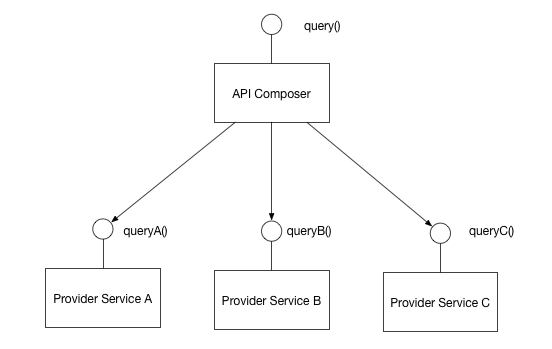
\includegraphics[width=.6\columnwidth]{./img/new/api_composition_pattern.png}%
	\end{center}
	\caption{API Composition паттерн}%
	\label{pic:api_composition_pattern}%
\end{figure}

\subsection{Способы взаимодействия между микросервисами}
Основные запросы которые будут поступать в ИИ ассистент врача, это запросы на получение того или иного ресурса. Данные запросы
реализуются посредством обычных синхронных интернет запросов, в API Composition. Далее из API Composition запросы передаются в микросервисы.


Однако стоит рассмотреть сценарий загрузки узи снимков на обработку в систему. Обработка узи снимка занимает значительное для пользователя время.
Нужен механизм, который избавит пользователя от необходимости активного ожидания результатов обработки узи снимка.\\
Решением этой проблемы - во время загрузки узи снимка, система ставит асинхронную задачу на обработку узи снимка. Если 
задача поставлена успешно, пользователь получает идентификатор задачи, после чего может посредством отдельных запросов узнать статус задачи.
В данном случае ожидание пользователя будет сведено к загрузке узи снимка.
В таком случае, схема начала обработки узи снимка будет выглядеть следующим образом:
\begin{figure}[H]%
	\begin{center}
		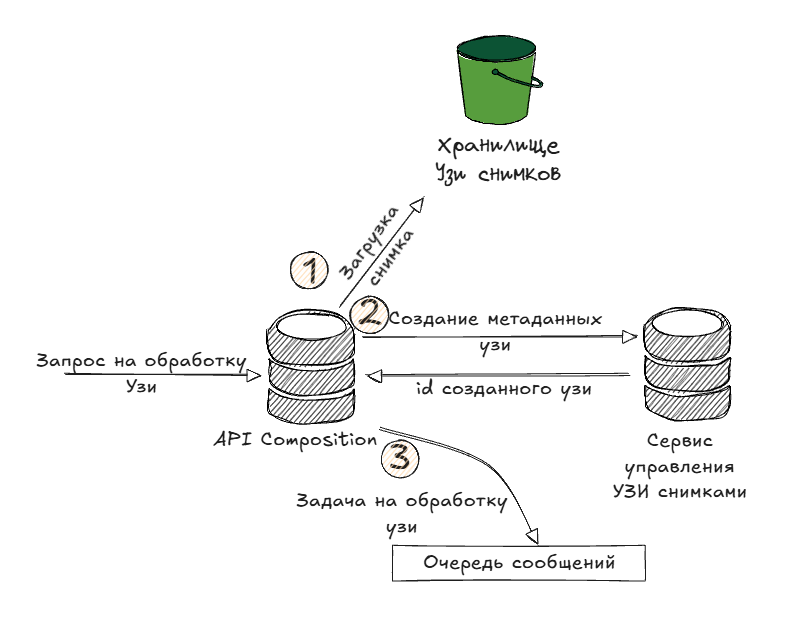
\includegraphics[width=.6\columnwidth]{./img/new/async.png}%
	\end{center}
	\caption{Схема асинхронной обработки узи снимка}%
	\label{pic:async}%
\end{figure}

\subsection{Итоговая архитектура системы Интеллектуального ассистента врача щитовидной железы}

Применяя паттерны API Composition при проектировании, а также учитывая синхронное и асинхронное взаимодействие между микросервисами,
мы получаем следующую архитектуру системы:
\begin{figure}[H]%
	\begin{center}
		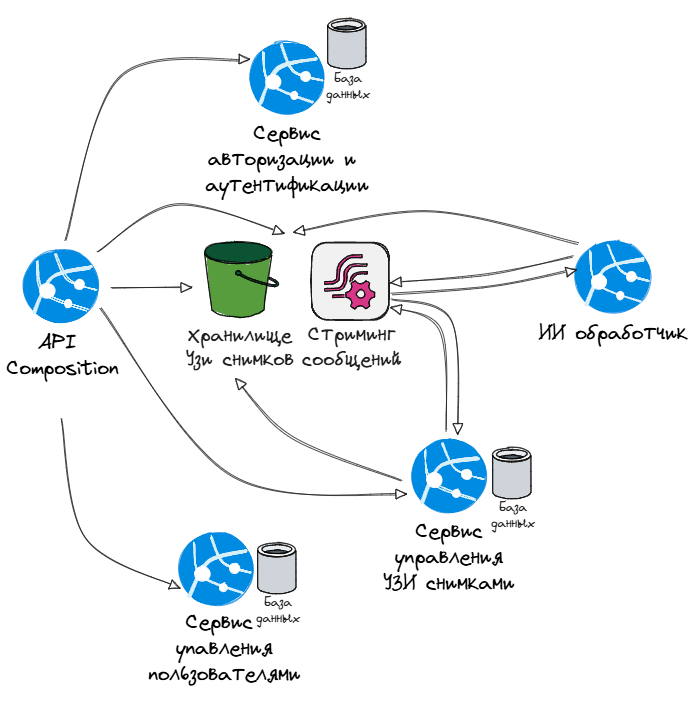
\includegraphics[width=.6\columnwidth]{./img/new/microservice_arch.png}%
	\end{center}
	\caption{Итоговая архитектура микросервисной системы}%
	\label{pic:microservice_arch}%
\end{figure}

\section{Выбор технологий и инструментов для технической реализации системы}

\subsection{Языка программирования}

\subsubsection*{Философия и дизайн языков}

\textbf{Python} следует философии простоты и читаемости кода, воплощённой в принципе \textit{"Zen of Python"}. Язык спроектирован так, чтобы код был максимально понятным и выразительным, что делает его идеальным для быстрого прототипирования и обучения программированию.

\textbf{Java} основан на принципах объектно-ориентированного программирования и философии \textit{"write once, run anywhere"}. Язык обеспечивает строгую типизацию и надёжность выполнения программ за счёт виртуальной машины Java (JVM).

\textbf{Go} создавался с целью объединить простоту синтаксиса с высокой производительностью. Разработчики Google стремились создать язык, который был бы эффективен для создания масштабируемых сетевых приложений и системного программирования.

\subsubsection*{Производительность и скорость выполнения}

По скорости выполнения языки располагаются в следующем порядке:

\begin{enumerate}
    \item \textbf{Go} --- компилируемый язык, обеспечивающий производительность, близкую к C/C++
    \item \textbf{Java} --- благодаря JIT-компиляции и оптимизациям JVM показывает высокую производительность
    \item \textbf{Python} --- интерпретируемый язык с относительно низкой скоростью выполнения
\end{enumerate}

Однако важно отметить, что Python компенсирует низкую скорость выполнения возможностью использования оптимизированных библиотек, написанных на C/C++, таких как NumPy и Pandas.

\subsubsection*{Синтаксис и удобство разработки}

\textbf{Python} обладает наиболее лаконичным и интуитивным синтаксисом. Отсутствие точек с запятой, использование отступов для обозначения блоков кода и богатая стандартная библиотека делают разработку быстрой и приятной.

\textbf{Java} требует больше \textit{boilerplate}-кода, но обеспечивает чёткую структуру и типобезопасность. Современные версии Java (начиная с Java 8) значительно упростили синтаксис благодаря лямбда-выражениям и другим нововведениям.

\textbf{Go} сочетает простоту синтаксиса с мощными возможностями. Язык имеет минималистичный дизайн, но при этом включает встроенную поддержку параллельного программирования через горутины и каналы.

\subsubsection*{Экосистема и библиотеки}

\textbf{Python} обладает самой обширной экосистемой для задач машинного обучения, науки о данных и веб-разработки. PyPI содержит сотни тысяч пакетов практически для любых задач.

\textbf{Java} имеет зрелую экосистему корпоративной разработки с такими фреймворками, как Spring, Hibernate, Apache Commons. Maven и Gradle обеспечивают надёжное управление зависимостями.

\textbf{Go} обладает растущей, но пока более ограниченной экосистемой. Встроенный пакетный менеджер и стандартная библиотека покрывают большинство базовых потребностей, особенно для сетевого и системного программирования.

\subsubsection*{Области применения}

\begin{description}
    \item[Python:] машинное обучение, анализ данных, веб-разработка (Django, Flask), автоматизация, скриптинг
    \item[Java:] корпоративные приложения, Android-разработка, веб-сервисы, большие распределённые системы
    \item[Go:] микросервисы, сетевые приложения, DevOps-инструменты, системное программирование
\end{description}

\subsubsection*{Параллельное программирование}

\textbf{Go} предоставляет наиболее элегантную модель параллельного программирования с горутинами и каналами, основанную на принципах CSP (Communicating Sequential Processes).

\textbf{Java} использует традиционную модель потоков с возможностями из пакета \texttt{java.util.concurrent}, а также современные решения вроде Project Loom.

\textbf{Python} ограничен Global Interpreter Lock (GIL), что затрудняет истинное многопоточное выполнение, хотя существуют способы обхода через multiprocessing и asyncio.


\textbf{Заключение}

Учитывая наши требования и специфику приложений, мы выбираем Golang как язык программирования для ассистента.

\subsection{Реляционные хранилища данных}
\textbf{Реляционные базы данных}: Реляционные базы данных, такие как MySQL и PostgreSQL, предлагают структурированный способ хранения данных с использованием таблиц, что позволяет легко реализовать связи между ними. Они подходят для большинства приложений, требующих согласованности и целостности данных.

\subsubsection*{Общая характеристика}

PostgreSQL и MySQL являются двумя наиболее популярными системами управления базами данных с открытым исходным кодом. Каждая из них имеет свои особенности и области применения.

\subsubsection*{Основные различия}

\textbf{Архитектура и подход}
PostgreSQL представляет собой объектно-реляционную СУБД, следующую стандартам SQL и поддерживающую сложные типы данных. MySQL изначально создавалась как быстрая и простая реляционная СУБД.

\textbf{Производительность}
MySQL традиционно показывает лучшие результаты в простых операциях чтения и веб-приложениях. PostgreSQL превосходит в сложных запросах, аналитике и операциях записи с высокой конкуренцией.

\textbf{Функциональность}
PostgreSQL предлагает расширенные возможности: поддержку JSON, массивов, пользовательских типов данных, оконных функций и процедурных языков. MySQL имеет более простой набор функций, но достаточный для большинства веб-приложений.

\subsubsection*{Области применения}

\textit{PostgreSQL} оптимален для:
\begin{itemize}
\item Сложных аналитических систем
\item Приложений с высокими требованиями к целостности данных
\item Проектов, требующих расширенной функциональности SQL
\end{itemize}

\textit{MySQL} предпочтителен для:
\begin{itemize}
\item Веб-приложений и CMS
\item Проектов с простыми запросами и высокой нагрузкой на чтение
\item Систем, где важна простота администрирования
\end{itemize}

\textbf{Заключение}

Учитывая наши требования и специфику приложений, мы выбираем PostgreSQL как основное решение для хранения данных в нашей архитектуре.

\subsection{Хранилище УЗИ снимков}

В современном мире информационных технологий выбор подходящей системы хранения данных становится критически важным решением. Каждый тип хранилища имеет свои особенности, преимущества и области применения. Рассмотрим три основных подхода к организации хранения данных.
\subsubsection*{Объектное хранилище}
Объектное хранилище представляет собой архитектуру, где данные хранятся в виде объектов в плоском пространстве имен. Каждый объект содержит сами данные, метаданные и уникальный идентификатор.
\textbf{Ключевые особенности:}
\begin{itemize}
\item Масштабируемость до петабайтов данных
\item REST API для доступа к данным
\item Отсутствие традиционной файловой иерархии
\item Встроенная репликация и обеспечение целостности данных
\end{itemize}
\textbf{Преимущества:}
\begin{itemize}
\item Практически неограниченная масштабируемость
\item Высокая надежность благодаря распределенной архитектуре
\item Экономическая эффективность для больших объемов данных
\item Идеально подходит для веб-приложений и API
\end{itemize}
\textbf{Недостатки:}
\begin{itemize}
\item Невозможность модификации объектов (только замена)
\item Более высокая латентность по сравнению с локальными системами
\item Ограниченная поддержка POSIX-операций
\end{itemize}
\textbf{Примеры использования:} Amazon S3, облачные сервисы, резервное копирование, хранение мультимедиа контента.
\subsubsection*{Файловое хранилище}
Традиционные файловые системы организуют данные в виде иерархической структуры папок и файлов. Это наиболее привычный и широко используемый подход к хранению данных.
\textbf{Ключевые особенности:}
\begin{itemize}
\item Иерархическая структура каталогов
\item Прямой доступ к файлам через файловую систему
\item Поддержка стандартных операций чтения/записи
\item Интеграция с операционными системами
\end{itemize}
\textbf{Преимущества:}
\begin{itemize}
\item Простота использования и понимания
\item Быстрый доступ к данным
\item Полная совместимость с существующими приложениями
\item Поддержка всех стандартных файловых операций
\end{itemize}
\textbf{Недостатки:}
\begin{itemize}
\item Ограниченная масштабируемость
\item Уязвимость к отказам оборудования
\item Сложность резервного копирования больших объемов данных
\item Производительность снижается при работе с миллионами файлов
\end{itemize}
\textbf{Примеры использования:} Локальные диски, NAS-системы, файловые серверы предприятий.
\subsubsection*{Распределенные файловые системы}
Распределенные файловые системы объединяют преимущества традиционного файлового хранилища с возможностями распределенной архитектуры, обеспечивая масштабируемость и отказоустойчивость.
\textbf{Ключевые особенности:}
\begin{itemize}
\item Данные распределены по множеству узлов
\item Прозрачный доступ к файлам как к локальным
\item Автоматическая репликация и восстановление
\item Горизонтальное масштабирование
\end{itemize}
\textbf{Преимущества:}
\begin{itemize}
\item Высокая доступность и отказоустойчивость
\item Масштабируемость путем добавления новых узлов
\item Сохранение привычного файлового интерфейса
\item Автоматическое распределение нагрузки
\end{itemize}
\textbf{Недостатки:}
\begin{itemize}
\item Сложность настройки и администрирования
\item Потенциальные проблемы с консистентностью данных
\item Зависимость от сетевой инфраструктуры
\item Более высокая стоимость внедрения
\end{itemize}
\textbf{Примеры использования:} Hadoop HDFS, GlusterFS, Ceph, высоконагруженные системы, big data аналитика.
\subsubsection*{Сравнительная таблица}

\begin{table}[H]
\centering
\begin{tabular}{|l|l|l|l|}
\hline
\textbf{Критерий}       & \textbf{Объектное}            & \textbf{Файловое}             & \textbf{Распределенные} \\ \hline
Масштабируемость        & Очень высокая                 & Малая                         & Высокая \\ \hline
Производительность      & Средняя                       & Высокая                       & Высокая \\ \hline
Надежность              & Очень высокая                 & Низкая                        & Высокая \\ \hline
Простота использования  & Средняя                       & Высокая                       & Низкая \\ \hline
Стоимость               & Низкая                        & Средняя                       & Высокая \\ \hline
\end{tabular}
\caption{Сравнение нереалиционных баз данных}
\end{table}

\subsubsection* {Выбор подходящего решения}
Выбор типа хранилища зависит от конкретных требований:
\textbf{Объектное хранилище} идеально для веб-приложений, резервного копирования и архивирования данных, где требуется высокая масштабируемость при умеренных требованиях к производительности.
\textbf{Файловое хранилище} остается оптимальным выбором для локальных приложений, небольших и средних объемов данных, где важна простота и производительность.
\textbf{Распределенные файловые системы} подходят для корпоративных решений с высокими требованиями к доступности и необходимостью обработки больших объемов данных с сохранением файлового интерфейса.
Современные IT-инфраструктуры часто используют гибридный подход, сочетая различные типы хранилищ в зависимости от специфики задач и требований к данным.

\subsection{Синхронное взаимодействие между микросервисами}

Микросервисы могут синхронно общаться между собой с использованием различных технологий и протоколов. 
В этом контексте рассмотрим четыре популярных метода взаимодействия: HTTP/REST API, gRPC, GraphQL и WebSocket.

В большинстве случаев для микросервисов, которые обмениваются фиксированными данными, использование GraphQL 
может быть излишним, поскольку этот подход предназначен для динамического запроса данных. В сценариях, 
где структуры данных заранее известны и не требуют изменения, REST API будет более простым и 
понятным решением. То же касается и WebSocket: двунаправленный стриминг данных может быть избыточным для 
многих бизнес-приложений, где достаточно стандартного запроса и ответа.

Таким образом, основные методы, которые стоит рассмотреть для синхронного взаимодействия микросервисов, — 
это HTTP/REST API и gRPC.


\textbf{HTTP/REST API}
HTTP/REST API — это один из самых распространенных способов синхронного взаимодействия между микросервисами. Каждый микросервис предоставляет набор эндпоинтов, к которым другие сервисы могут обращаться для выполнения операций и получения данных. Используя стандартные методы HTTP (GET, POST, PUT, DELETE), микросервисы обмениваются сообщениями с четко определенными правилами и структурой.


\textbf{Преимущества использования HTTP/REST}
\begin{itemize}
    \item \textbf{Простота}: REST API легко реализовать и документировать. Он основан на понятных стандартах HTTP и может использоваться практически на любой платформе.
    \item \textbf{Читаемость}: Структура URL и использование HTTP-методов делают интерфейс API интуитивно понятным и удобным для работы разработчиков.
    \item \textbf{Совместимость}: REST API может легко взаимодействовать с разными языками программирования и платформами, что делает его универсальным решением для микросервисной архитектуры.
\end{itemize}


\textbf{gRPC}
gRPC, разработанный Google, представляет собой высокопроизводительный фреймворк для удаленных вызовов процедур (RPC), который поддерживает множество языков программирования. Он использует HTTP/2 для передачи данных, что обеспечивает преимущества, такие как многопоточность и меньшие задержки при передаче информации.


\textbf{Преимущества использования gRPC}
\begin{itemize}
    \item \textbf{Производительность}: Использование HTTP/2 позволяет gRPC эффективно обрабатывать множество параллельных запросов, что делает его более производительным, чем традиционные REST API.
    \item \textbf{Статическая типизация}: gRPC использует Protocol Buffers для описания структуры данных, что позволяет разработчикам строго определять, какой тип данных будет передаваться. Это обеспечивает дополнительную безопасность и позволяет избежать ошибок при взаимодействии между сервисами.
    \item \textbf{Автогенерация кода}: Удобство разработки достигается благодаря автоматической генерации клиентского кода на разных языках, что ускоряет процесс создания микросервисов.
\end{itemize}


\textbf{Сравнение HTTP/REST API и gRPC}
\begin{table}[h]
    \centering
    \begin{tabular}{|l|l|l|}
        \hline
        \textbf{Характеристика}           & \textbf{HTTP/REST API}                          & \textbf{gRPC}                                     \\ \hline
        Протокол                  & HTTP/1.1            & HTTP/2                             \\ \hline
        Структура данных          & JSON/XML                        & Protobuff \\ \hline
        Типизация                 & Динамическая            & Статическая  \\ \hline
        Производительность         & Низкая         & Высокая \\ \hline
        Поддержка потоковой передачи & Ограниченная                                & Полная \\ \hline
        Автогенерация клиента     & Нет & Да \\ \hline
    \end{tabular}
    \caption{Сравнение HTTP/REST API и gRPC}
\end{table}


\textbf{Заключение}
Нашей системе не требуется возможность динамической типизации, поэтому выбор сделать в сторону gRPC.

\subsection{Асинхронное взаимодействие} % kafka

Асинхронное взаимодействие между микросервисами позволяет увеличить производительность и гибкость распределенных систем. В этом подходе микросервисы могут обмениваться данными без необходимости дожидаться ответа, что снижает задержки и повышает общую эффективность системы. Рассмотрим основные методы асинхронного взаимодействия.

\textbf{Основные методы асинхронного взаимодействия}
\begin{itemize}
    \item \textbf{Очереди сообщений}: Использование систем обмена сообщениями, таких как RabbitMQ, Apache Kafka или Redpanda, позволяет отправлять сообщения между микросервисами без прямого связывания. Один сервис может отправлять сообщения в очередь, а другой — извлекать их и обрабатывать по мере возможности. Это гарантирует, что сервисы могут работать независимо друг от друга и не блокируют друг друга в случае высокой нагрузки.
    \item \textbf{Событийно-ориентированная архитектура}: В этой архитектуре микросервисы реагируют на события, происходящие в системе. События могут генерироваться различными компонентами и служить сигналами для других микросервисов о том, что произошло что-то важное (например, изменение состояния, завершение задачи и т. д.). Это позволяет строить более гибкие и масштабируемые системы.
    \item \textbf{HTTP-события (Webhooks)}: Использование вебхуков позволяет микросервису отправлять HTTP-запросы в другие сервисы при наступлении определённых событий. Это простой способ интеграции, позволяющий уведомлять другие службы о произошедших изменениях или событиях.
\end{itemize}

Выбор в сторону очередей сообщений также обуславливается необходимостью наличия механизма Dead Letter Queue (DLQ), который позволяет обрабатывать ошибки при отправке и получении сообщений. Кроме того, мы стремимся автоматизировать хранение сообщений, что делает использование очередей сообщений предпочтительным решением.

\textbf{Описание систем очередей сообщений}
\begin{itemize}
    \item \textbf{Apache Kafka}:
            - Kafka — это распределенная платформа для потоковой передачи данных, которая обеспечивает высокую пропускную способность и низкую задержку. Она работает по принципу публикации и подписки, позволяя множеству клиентов читать и писать сообщения.
            - \textbf{Назначение}: Идеально подходит для обработки потоков данных в реальном времени и хранения больших объемов событий с возможностью их долговременного хранения.
    \item \textbf{Redpanda}:
            - Redpanda — это высокопроизводительная, совместимая с Kafka, распределенная система сообщений, оптимизированная для работы с потоками данных в реальном времени.
            - \textbf{Назначение}: Обеспечивает низкую задержку и простоту настройки, что делает её предпочтительной для решений, требующих высокой производительности. 
    \item \textbf{Apache Pulsar}:
            - Pulsar — это распределенная система потоковой передачи данных, которая поддерживает многопоточность и управление потоками. Она предоставляет гибкий подход к очередям сообщений и событиям.
            - \textbf{Назначение}: Отличается поддержкой долгосрочного хранения сообщений и сложных сценариев работы с геораспределёнными данными.
\end{itemize}

\textbf{Заключение}
Асинхронное взаимодействие, организованное через очереди сообщений, является эффективным способом повышения производительности и устойчивости микросервисов. Учитывая возможности по снижению задержки и простой настройке, мы выбрали Redpanda как предпочтительное решение для организации асинхронного взаимодействия между микросервисами.

\section{Выводы}


\begin{enumerate}
	\item Разработана оптимизированная микросервисная архитектура с применением паттерна API Composition, минимизирующего зависимости между компонентами системы.
    \item Сформирован технологический стек реализации: Golang (основной язык), PostgreSQL (реляционное хранилище), объектное хранилище minio S3 (для УЗИ-данных), gRPC (синхронное взаимодействие) и Redpanda (асинхронные очереди)
    \item Реализованы специализированные механизмы взаимодействия, включая асинхронную модель обработки УЗИ-снимков с возвратом идентификатора задачи и поддержкой Dead Letter Queue для устойчивой работы
\end{enumerate}

% В этой главе описывается, что и как было спроектировано. 
% При необходимости, описывается использованная методика проектирования. 
% Сюда же относится описание внешних и внутренних программных интерфейсов, 
% а также форматы и структуры входных и выходных данных.


% \section{Использование методики <<такой-то>> для проектирования программных систем <<такого-то типа>>}

% \dots

% \section{Общая архитектура системы \dots}

% \dots


% Команда \texorpdfstring необходима, чтобы программа просмотра PDF документов
% верно отображала текст формул в панели оглавления.
% При отсутствии команды \texorpdfstring там, где она необходима, LaTeX выводит
% предупреждение "Token not allowed in a PDF string"
% \section{Архитектура подсистемы \texorpdfstring{$1$}{1}\dots}

% \dots


% \section{Архитектура подсистемы \texorpdfstring{$N$}{N}\dots}

% \dots


% \section{
%   Проектирование протокола взаимодействия подсистем \texorpdfstring{$X$}{X} и
%   \texorpdfstring{$Y$}{Y}
% }

% \dots


% \section{Выводы}

% Следует перечислить, какие инженерные результаты были получены, а именно: 
% какие программные системы, подсистемы или модули были спроектированы. Следует 
% не только назвать полученные архитектуры, но и отметить их отличительные 
% особенности.

%%% Local Variables:
%%% TeX-engine: xetex
%%% eval: (setq-local TeX-master (concat "../" (seq-find (-cut string-match ".*-3-pz\.tex$" <>) (directory-files ".."))))
%%% End:


\clearpage

\chapter{Реализация и тестирование системы}

\section{Реализация компонентов системы в виде микросервисов}

\subsection{Сущности предметной области}
В каждом микросервисе существует своя предметная область. Все ключевые сущности заданы в виде структур, для оперирования
ими в логике микросервиса.

\begin{figure}[H]%
	\begin{center}
		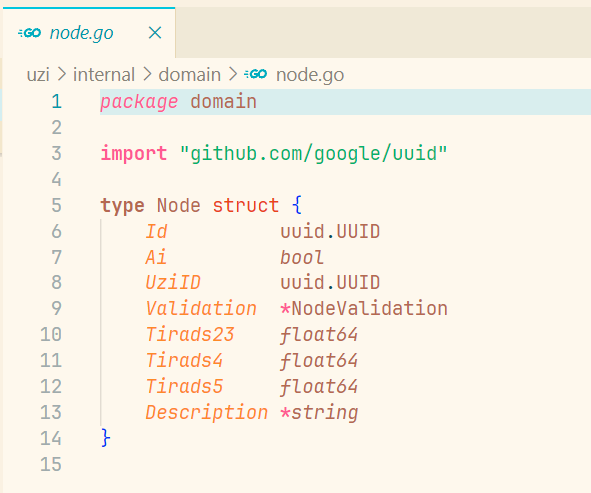
\includegraphics[width=.7\columnwidth]{./img/new/domain_node.png}%
	\end{center}
	\caption{Сущности узла образования в щитовидной железе}%
	\label{pic:domain_node}%
\end{figure}

\begin{figure}[H]%
	\begin{center}
		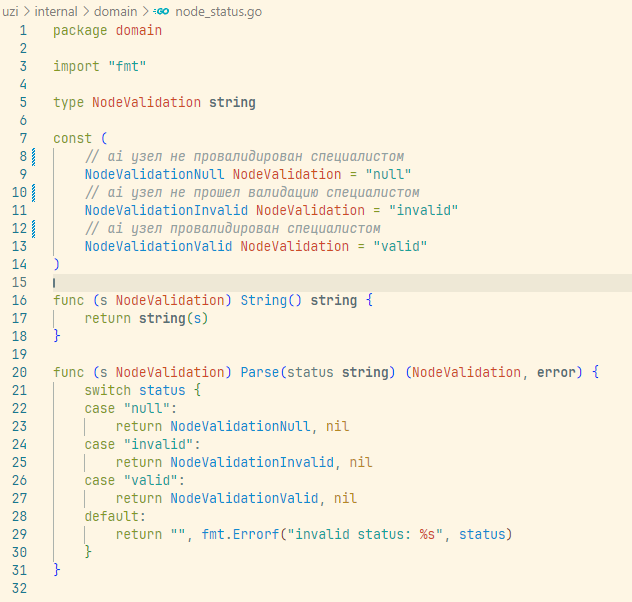
\includegraphics[width=.7\columnwidth]{./img/new/domain_node_status.png}%
	\end{center}
	\caption{Статусы узла образования в щитовидной железе}%
	\label{pic:domain_node_status}%
\end{figure}

Сущности предметной области не имеют зависимостей от внешних частей или структур системы.

\subsection{Логические сценарии использования}
Вся логика которая имеется в микросервисе реализована в этом слое приложения. Никакая логика не допустима в другом месте. 
Такой подход к разработке позволяет легко отлаживать и контролировать систему, она не <<растякается>> по всему коду.

\begin{figure}[H]%
	\begin{center}
		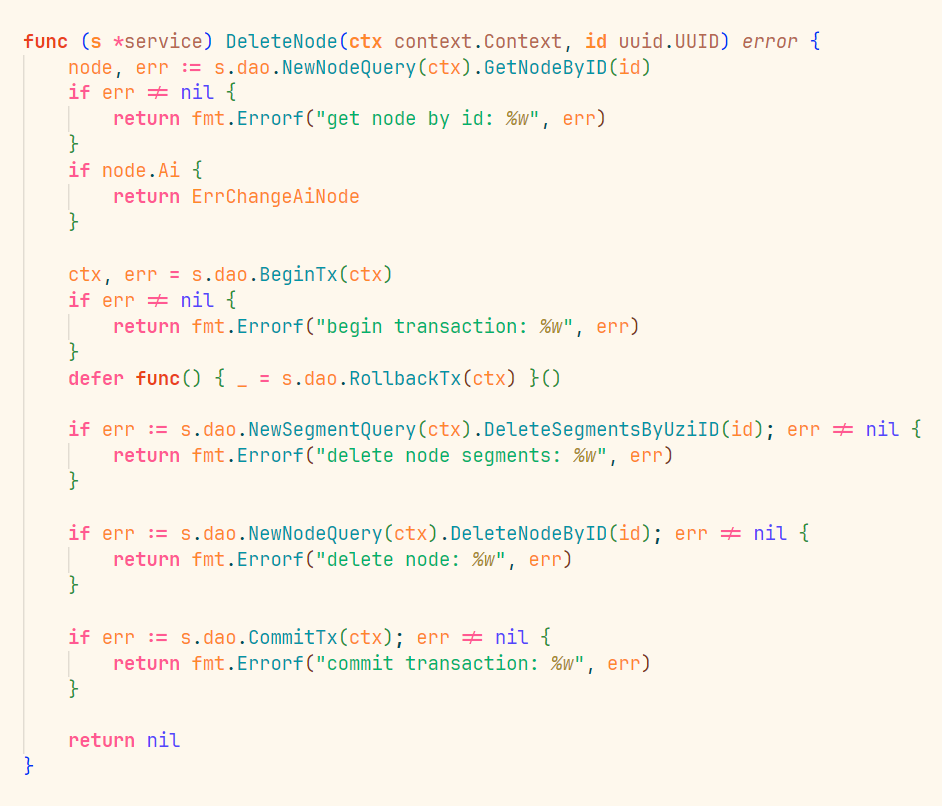
\includegraphics[width=.7\columnwidth]{./img/new/logical.png}%
	\end{center}
	\caption{Логическая удаления узла образования}%
	\label{pic:logical}%
\end{figure}

\subsection{Интерфейсы взаимодействия с внешними системами}
Для сохранения правила Dependency Inversion, все взаимодействия с внешними системами реализованы через интерфейсы, чей уровень
абстракции такого же уровня, что и уровень абстракции вызывающего интерфейс. Рассмотрим пример интерфейса для взаимодействия с 
базой данных.

\begin{figure}[H]%
	\begin{center}
		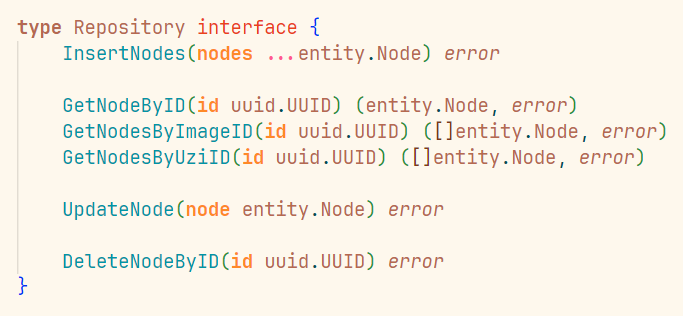
\includegraphics[width=.7\columnwidth]{./img/new/repository.png}%
	\end{center}
	\caption{Интерфейс взаимодействия с базой данных для узлов образований}%
	\label{pic:repository}%
\end{figure}

\subsection{Контракты микросервисов и API системы}
Все микросервисы взаимодействуют с друг другом посредством gRPC. Описания контрактов взаимодействия делается посредством
proto файлов. В них описываются rpc методы микросервиса, которые он реализует. Описаны ожидаемые структуры данных, которые 
используются в rpc методах.

\begin{figure}[H]%
	\begin{center}
		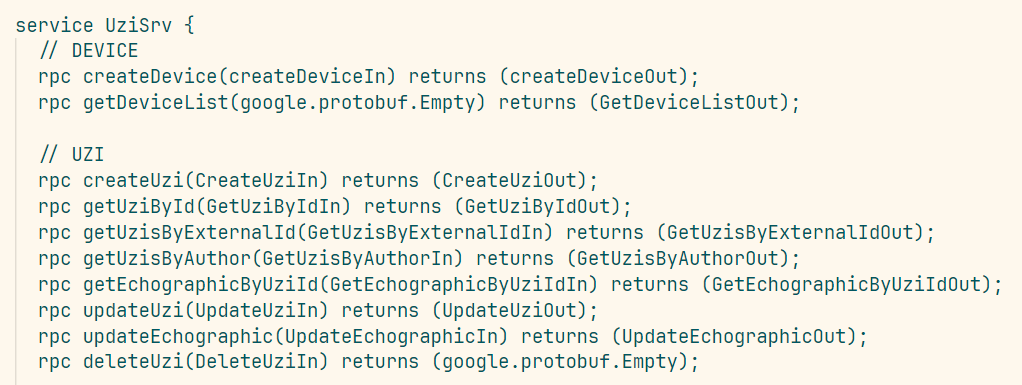
\includegraphics[width=.7\columnwidth]{./img/new/rpc_proto_1.png}%
	\end{center}
	\caption{Контракт взаимодействия с микросервисом управления УЗИ снимками}%
	\label{pic:rpc_proto_1}%
\end{figure}

\begin{figure}[H]%
	\begin{center}
		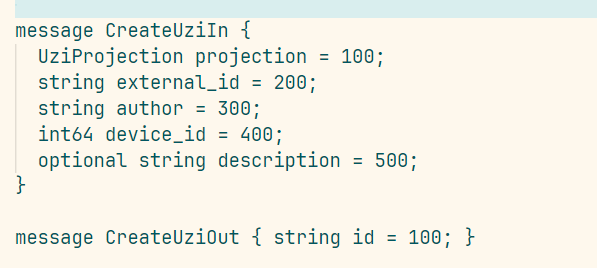
\includegraphics[width=.7\columnwidth]{./img/new/rpc_proto_2.png}%
	\end{center}
	\caption{Контракт взаимодействия с микросервисом управления УЗИ снимками}%
	\label{pic:rpc_proto_2}%
\end{figure}

Далее рассмотрим API системы в целом. Этот API должен в полной мере покрывать все функциональные требования к системе, 
относящиеся к взаимодействию с системой. API системы описывается файлом в формате OpenAPI 3.0.

\begin{figure}[H]%
	\begin{center}
		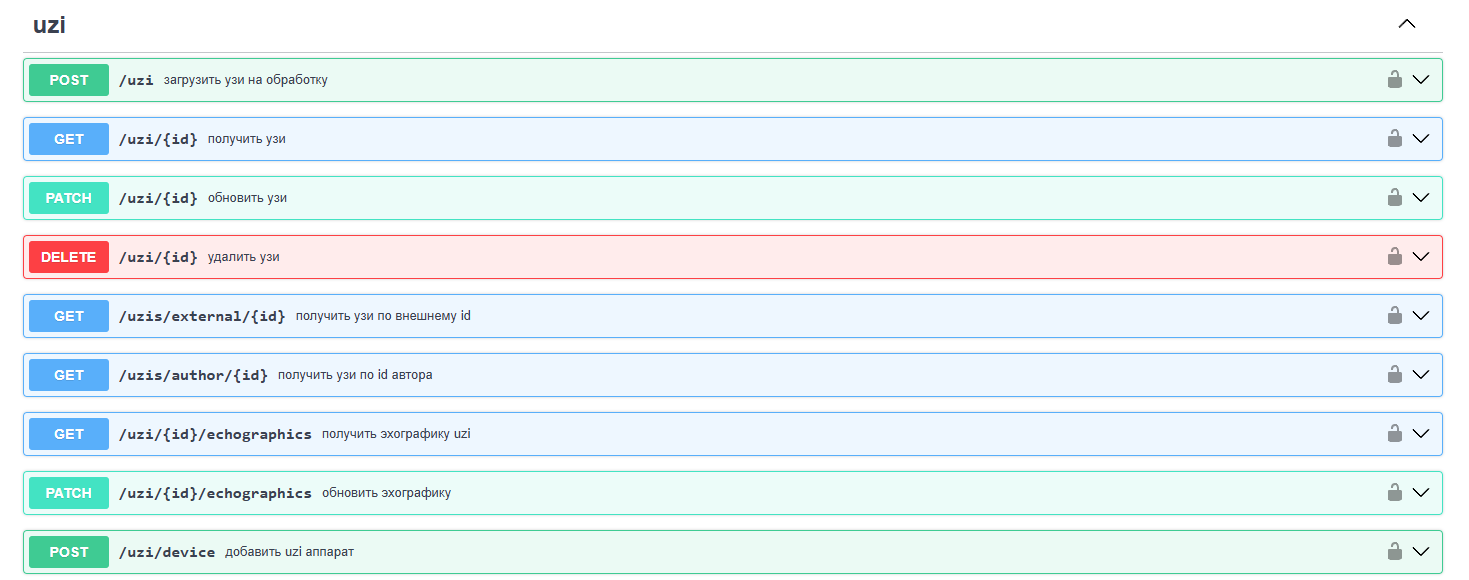
\includegraphics[width=.7\columnwidth]{./img/new/swagger_small.png}%
	\end{center}
	\caption{API системы}%
	\label{pic:swagger_small}%
\end{figure}

\subsection{Топики стриминга сообщений для асинхронного общения}
Для использования асинхронного общения через RedPanda, создадим 3 топика:
\begin{itemize}
    \item \textbf{uziupload} - узи загруженно в S3. Запустит разбиение узи на кадры.
    \item \textbf{uzisplitted} - узи разбито на кадры. Запустит обработку узи нейро моделью. В топик пишет сервис управления УЗИ после разбиения узи на кадры.
    \item \textbf{uziprocessed} - узи обработанно нейромоделью. Узи сегментировано и классифицировано
\end{itemize}

\subsection{Структура хранилища узи снимков}
Структура S3 minio представлена в виде файловой системы, позволяет быстро искать необходимые файлы, зная их идентификатор. 
Микросервисы знают об устройстве S3, поэтому при необходимости передчи в другой микросервис узи снимков, достаточно передавать
id снимка.

\begin{figure}[H]%
	\begin{center}
		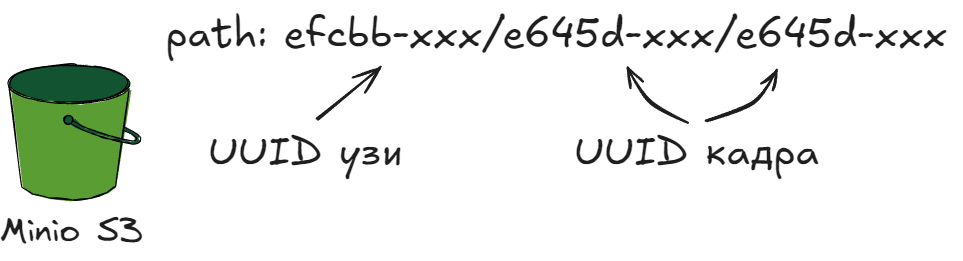
\includegraphics[width=.6\columnwidth]{./img/s3_arc.png}%
	\end{center}
	\caption{Структура S3 хранилища}%
	\label{pic:auth_model}%
\end{figure}


% В этой главе описывается, что и как было запрограммировано, отлажено, 
% протестировано, и что в результате получилось. Большинство работ должны 
% содержать приведенные ниже разделы. Но нужно учитывать, что точный состав 
% этой главы, как и других глав, зависит от специфики работы.

% Фрагменты программного кода в тексте необходимо выделять при помощи команды 
% \verb|\verb|. Многострочные листинги должны оформляться при помощи пакета 
% \verb|listings|. Пример:

% \begin{lstlisting}
% # let s x y z = x z (y z);;
% val s : ('a -> 'b -> 'c) -> ('a -> 'b) -> 'a -> 'c = <fun>
% # let k x y = x;;
% val k : 'a -> 'b -> 'a = <fun>
% # let i = s k k;;
% val i : '_a -> '_a = <fun>
% \end{lstlisting}

% Листинг \ref{lst:float-example} иллюстрирует использование выносных листингов.
% Листинг \ref{lst:HelloWorld.scala} показывает пример включения внешнего файла 
% в качестве листинга, в данном случае --- выносного.

% \begin{lstlisting}[
%   float=tb,frame=lines,label=lst:float-example,caption=Выносной листинг
% ]
% List myList = new List();
% Element myElement = new Element();
% myList.Append(myElement);
% \end{lstlisting}

% \lstinputlisting[
%   label=lst:HelloWorld.scala,
%   float=tb,frame=lines,
%   caption=Листинг из файла \texttt{HelloWorld.scala}
% ]{listings/HelloWorld.scala}


\section{Состав и структура реализованного программного обеспечения}

Реализованно серверное приложение, запускаемое как для локального использование, так и в 
серверном виде. Приложений отвечает на HTTP запросы, соответствует всем функциональным требованиям к системе.

\subsection{Структура приложения}
Приложение состоит из 5 микросервисов:
\begin{itemize}
  \item Composition API - точка входа в систему. Обрабатывает запросы от пользователя и передает их в соответствующие микросервисы.
  \item Микросервис Авторизации и Аутентификации - отвечает за аутентификацию и авторизацию пользователей.
  \item Микросервис Управления УЗИ снимками - отвечает за загрузку, разбиение на кадры, обработку узи нейромоделью.
  \item Микросервис Управления Медицинскими данными - отвечает за хранение и обработку медицинских данных.
  \item Микросервис Интеллектуальной части - отвечает за обработку узи нейромоделью.
\end{itemize}

Каждый микросервис написанный на golang содержит:
\begin{itemize}
  \item go.mod и go.sum файлы, описывающие библиотекчные зависимости для приложения
  \item sql файлы миграций. Сами миграции осуществлялись за счет утилиты Goose. SQL файлы в каждом микросервисе расположены по пути db/migrations
  \item proto файлы описывающие контракты для взаимодествия с внешними системами
  \item taskfile - файлы описывающие команды необходимые для локальной сборки микросервиса, миграции базы данных, генерации кода и т.д
  \item Dockerfile - файл для сборки docker образа микросервиса
  \item service.yml - файл содержащий конфигурацию сервиса
\end{itemize}


% Нужно охарактеризовать реализованное ПО: является ли оно настольной программной для Windows, 
% или веб-приложением в форме сайта/веб-сервиса, или модулем/подключаемой библиотекой, или 
% \dots. Также нужно перечислить, из чего оно состоит: какие исполняемые файлы и их назначение, 
% конфигурационные файлы, файлы баз данных, требования к программному и аппаратному окружению, и т.п.

% Если реализованное приложение достаточно обширно, этот раздел может быть
% разделен на несколько: один с общим описанием, и по одному на подсистемы самого
% верхнего уровня.

\section{Основные сценарии работы пользователя}
Основной сценарий работы ПО - отправка запросов на обработку узи изображений и полученние данных с
обработанных изображений. Для взаимодействием с сервисом предоставляется подробное swagger api.
\begin{figure}[H]%
	\begin{center}
		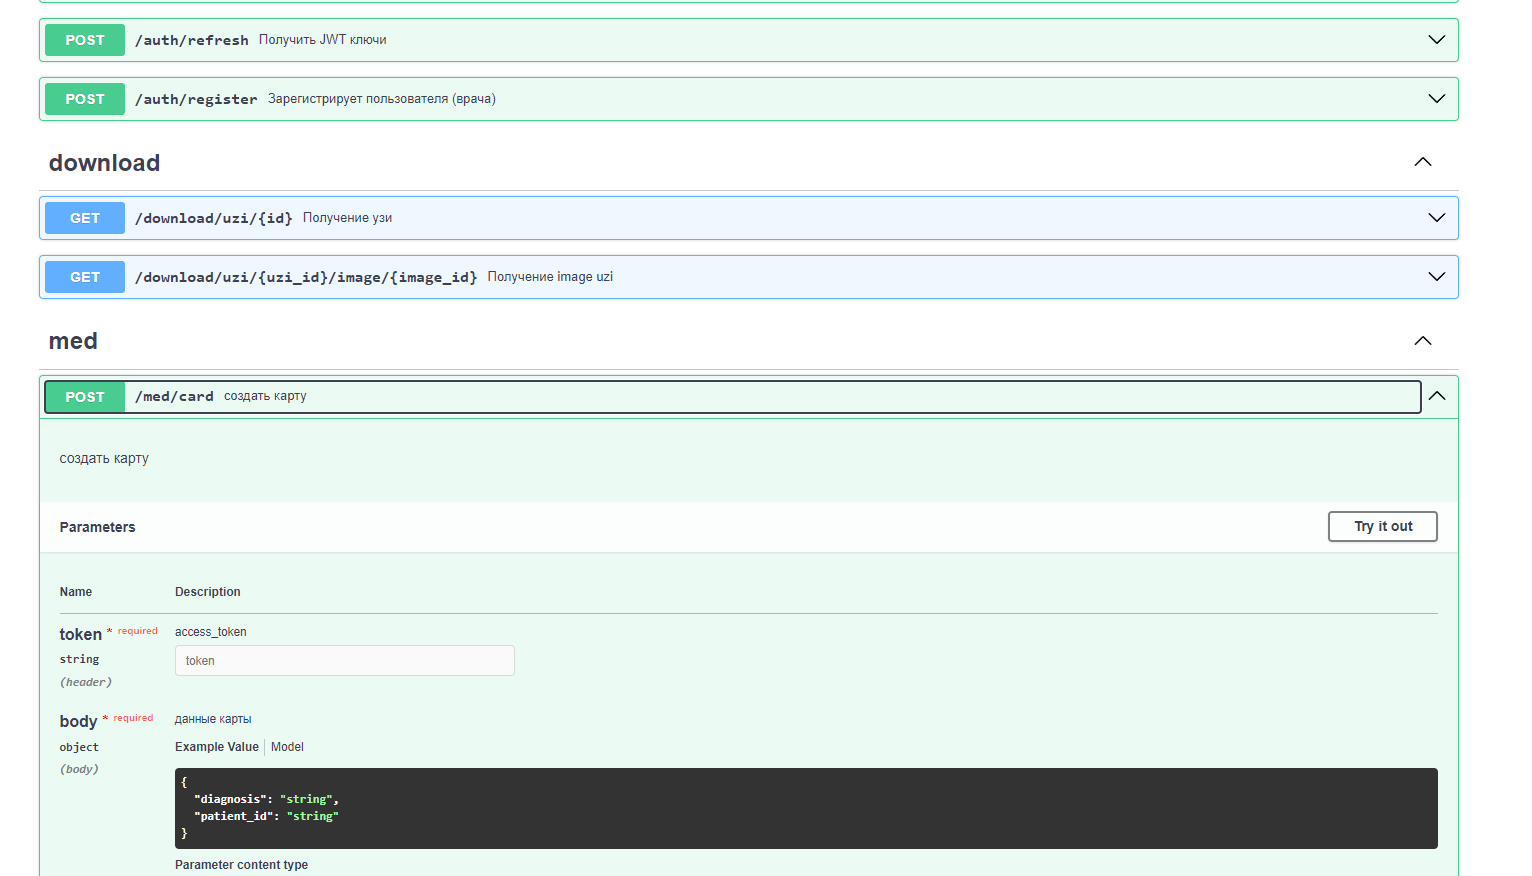
\includegraphics[width=.9\columnwidth]{./img/swagger.png}%
	\end{center}
	\caption{Спроектированная база данных Auth Service}%
	\label{pic:auth_model}%
\end{figure}

% Нужно помнить, что пользователем может быть не только <<менеджер>> или <<человек в белом халате>>, 
% но и другой программист. Последнее относится, в первую очередь, к реализованным библиотекам. 
% Для <<обычных>> приложений нередко бывают пользователи нескольких категорий --- например, обычный 
% пользователь и администратор. Для каждой категории нужно описать, как выполняются основные функции, 
% предпочтительно, с помощью серии скрин-шотов. Однако считается плохим тоном вставлять длинную вереницу 
% из скрин-шотов: если их много, большую часть нужно выносить в приложение. Для \textit{этого} раздела 
% нормальной является плотность скрин-шотов из расчета: 1 страница скрин-шотов на 1-2 страницы текста.


\section{Выводы}
Таким образом, в рамках НИРа было реализовано 4 микросервиса серверного приложения, а также были проведены некоторые типы тестирования реализации. 
В будущем планируется развернуть систему на нескольких физическим машинах с использованием оркестратора контейнеризированных приложений 
kubernetus и повторно провести нагрузочное и интеграционное тестирование.

% Следует перечислить, какие практические результаты были получены, а именно: какое 
% программное или иное обеспечение было создано. В число результатов могут входить, 
% например, методики тестирования, тестовые примеры (для проверки корректности/оценки 
% характеристик тех или иных алгоритмов) и др. По каждому результату следует сделать вывод, 
% насколько он отличается от известных промышленных аналогов и исследовательских прототипов.



%%% Local Variables:
%%% TeX-engine: xetex
%%% eval: (setq-local TeX-master (concat "../" (seq-find (-cut string-match ".*-3-pz\.tex$" <>) (directory-files ".."))))
%%% End:


\clearpage

\chapter*{Заключение}
\addcontentsline{toc}{chapter}{Заключение}

В аналитической части: 



\begin{enumerate}
	\item Выполнен анализ архитектурных стилей построения систем, с учетом требований к динамической расширяемости отдельных модулей системы, выбрана микросервисная архитектура с применением API Gateway.
	\item Проанализированы основные архитектурные паттерны построения приложений. Clean Architecture за счет преобраладания SOLID, разбиения на слои и преимуществ Dependency inversion выбрана как основа написания микросервисов.
	\item Проанализированных основные инструменты для разработки системы, произведены сравнения аналогов\\
        - для синхронного взаимодействия между микросервисами выбран gRPC, за счет строгой типизации контрактов и производительности за счет сериализации данных.\\
        - для асинхронного взаимодействия между микросервисами выбран подход с брокером сообщений, за счет универсальности и отказоустойчивости. В качестве реализации выбрана RedPanda, Kafka совместимое API с наибольшей производительностью.\\
        - для хранения структурированных данных выбрана PostgreSql, за счет развитой надежности и удобства\\
        - для хранения неструтурированных данных выбрано NoSQL хранилище S3 Minio.\\
        - в качестве схемы авторизации выбрана схема с JWT токенами, которая позволяет не хранить активное состоянии на серверной стороне.\\
\end{enumerate}


В теоретической части:


Были спроектированы модели Auth Service, Uzi Service и Gateway Service. Объединением всех этих моделей является
модель самой системы. Модели соответствуют и учитывают все функциональные требования к модулям системы и системе в целом.


В проектировании:


В результате были спроектированы модули системы и правила их взаимодействия с учетом выбранных средств разработки
на этапе анализа.


В итоге:


Таким образом, в рамках НИРа было реализовано 4 микросервиса серверного приложения, а также были проведены некоторые типы тестирования реализации. 
В будущем планируется развернуть систему на нескольких физическим машинах с использованием оркестратора контейнеризированных приложений 
kubernetus и повторно провести нагрузочное и интеграционное тестирование.

%%% Local Variables:
%%% TeX-engine: xetex
%%% eval: (setq-local TeX-master (concat "../" (seq-find (-cut string-match ".*-3-pz\.tex$" <>) (directory-files ".."))))
%%% End:


\label{end_of_main_text}

\setcounter{totalfigures}{\the\value{totalfigures}+\the\value{figure}}
\setcounter{figure}{0}
\setcounter{totaltables}{\the\value{totaltables}+\the\value{table}}
\setcounter{table}{0}
\setcounter{totallistings}{\the\value{totallistings}+\the\value{lstlisting}}
\setcounter{lstlisting}{0}

\makeatletter
\edef\@currentlabel{\the\value{totalfigures}}
\label{figures}
\edef\@currentlabel{\the\value{totaltables}}
\label{tables}
\edef\@currentlabel{\the\value{totallistings}}
\label{listings}
\makeatother

\clearpage

\input{chapters/thesis-template-bibl.tex}

\endrefsection

\clearpage

%\chapter*{Приложения}
%\addcontentsline{toc}{chapter}{Приложения}
%\appendixtocon
%\renewcommand{\appendixname}{Приложение}
\appendix
\renewcommand{\appendixtocname}{Приложения}
\addappheadtotoc
%\titleformat{\chapter}[block]{\centering\normalfont\Large\bfseries}{\chaptername{} \thechapter.}{1ex}{}{}
\renewcommand{\chaptername}{Приложение}
%\renewcommand*\printchaptername{\Large\bfseries\appendixname~}
%\renewcommand{\thechapter}{Приложение \Alph{chapter}}
%\renewcommand{\thechaptertoc}{Приложение \Alph{chapter}}

%\renewcommand{\chaptermark}[1]{\markboth{\chaptername\ \thechapter.\ #1}{}}

%\begin{appendices}
\chapter{Основные части компонента управление УЗИ снимками}\label{app-format}
%\addcontentsline{toc}{chapter}{}

\lstinputlisting[
  label=lst:uzi_service.proto,
  float=tb,frame=lines,
  caption=Контракт компонента управление УЗИ снимками
]{listings/uzi_service.proto}

\lstinputlisting[
  label=lst:uziupload.proto,
  float=tb,frame=lines,
  caption=Листинг топика \texttt{uziupload}
]{listings/uziupload.proto}

\lstinputlisting[
  label=lst:uzisplitted.proto,
  float=tb,frame=lines,
  caption=Листинг топика \texttt{uzisplitted}
]{listings/uzisplitted.proto}

\lstinputlisting[
  label=lst:uziprocessed.proto,
  float=tb,frame=lines,
  caption=Листинг топика \texttt{uziprocessed}
]{listings/uziprocessed.proto}

\lstinputlisting[
  label=lst:node_controller_hadnler.go,
  float=tb,frame=lines,
  caption=Контроллер gRPC ручек для взаимодействия с узлами
]{listings/node_controller_hadnler.go}

\lstinputlisting[
  label=lst:node_get_handler.go,
  float=tb,frame=lines,
  caption=Контроллер gRPC ручки получения узла узи
]{listings/node_get_handler.go}

\lstinputlisting[
  label=lst:create_nodes_1.go,
  float=tb,frame=lines,
  caption=Создание нового узла с сегментами ч.1
]{listings/create_nodes_1.go}

\lstinputlisting[
  label=lst:create_nodes_2.go,
  float=tb,frame=lines,
  caption=Создание нового узла с сегментами ч.2
]{listings/create_nodes_2.go}

\lstinputlisting[
  label=lst:uzi_1.sql,
  float=tb,frame=lines,
  caption=Создание бд узи компонента ч.1
]{listings/uzi_1.sql}

\lstinputlisting[
  label=lst:uzi2.sql,
  float=tb,frame=lines,
  caption=Создание бд узи компонента ч.2
]{listings/uzi2.sql}




% Текст пояснительной записки должен готовиться для печати на листах формата А4, использоваться должен шрифт с засечками (Roman; обычно --- Times Roman или Times New Roman), 12 или 14 кегль. Размеры полей:

% \begin{itemize}
% 	\item верхнее: 20 мм.
% 	\item нижнее: 20 мм.
% 	\item левое: 10 мм.
% 	\item правое: 25 мм.
% \end{itemize}

% Нумероваться должны все страницы, начиная с первой (титульной), однако сами номера следует проставлять на страницах, начиная со страницы реферата. Номер следует проставлять внизу страницу (в центре).

% Заголовки оформляются тем же шрифтом, что и основной текст (т.е., соответственно, Times Roman или Times New Roman). Для заголовков первого уровня размер шрифта может быть больше размера шрифта основного текста (обычно 14-16).

% Все разделы текста: реферат, оглавление, введение, три главы основного
% содержания, список литературы, заключение, приложения --- должны снабжаться
% содержательным заголовком и начинаться с новой страницы; сами заголовки следует
% при этом центрировать (заголовки параграфов и пунктов выравниваются по ширине).
% Следует обратить внимание, что заголовки всех разделов, кроме трех основных
% глав, регламентированы; заголовки трех основных глав должны быть содержательными
% и отражать суть соответствующей главы. Названия типа <<Аналитическая часть>> и <<Теоретическая глава>> --- \textit{недопустимы}.

% Текст пояснительной записки может содержать рисунки и таблицы. Все рисунки и
% таблицы должны снабжаться номерами и подписями:

% \begin{itemize}

% 	\item нумерация рисунков и таблиц должна быть сквозная (но раздельная, т.к. для рисунков своя, для таблиц --- своя);

% 	\item в случае большого количества иллюстраций/таблиц, допускается <<вложенная>> нумерация (т.е. таблицу/рисунок можно снабжать составным номером в формате 
	
% 	$$\langle\mbox{номер главы}\rangle.\langle\mbox{номер внутри главы}\rangle;$$
	
% 	\item подрисуночная подпись должна располагаться снизу по центру;
	
% 	\item название таблицы следует помещать над таблицей слева, без абзацного
% 	отступа в одну строку с ее номером через тире (ГОСТ 7.32-2001, п.6.6.1).

% \end{itemize}

% Здесь перечислены не все, а лишь основные требования к оформлению. Прочие
% требования --- см. соответствующие ГОСТы.

% Для того чтобы избежать больших отступов в списках, которые по умолчанию добавляют окружения \texttt{itemize} и \texttt{enumerate}, следует использовать 
% \texttt{compactitem} (для маркированных списков) и \texttt{compactenum} (для нумерованных списков) из пакета \texttt{paralist}. 
% Например:

% \begin{compactitem}
% 	\item это;
% 	\item не нумерованный;
% 	\item список;
% 	\item без лишних промежутков.
% \end{compactitem}

% И для нумерованных списков:

% \begin{compactenum}[1)]
% 	\item нумерованные списки;
% 	\item пакета \texttt{paralist};
% 	\item еще и удобно настраивать;
% 	\item (например, менять формат номера).
% \end{compactenum}

% \noindent или

% \begin{compactenum}[a)]
% 	\item это другой;
% 	\item нумерованный;
% 	\item список;
% 	\item без лишних промежутков;
% 	\item и с буквенной нумерацией.
% \end{compactenum}

% А если хочется нумерацию сделать ангоязычной, то нужно использовать окружение \texttt{other\-language} (таким образом: \verb|\begin{otherlanguage}[numerals=latin]{russian}|)

% \setkeys{russian}{numerals=latin}
% %\selectlanguage{russian}
% %\begin{otherlanguage}[numerals=latin]{russian}
% \begin{russian}
% \begin{compactenum}[a)]
% 	\item это другой;
% 	\item нумерованный;
% 	\item список;
% 	\item без лишних промежутков;
% 	\item и с буквенной нумерацией.
% \end{compactenum}
% \end{russian}
% %\end{otherlanguage}

% \textbf{Замечание.} По неизвестным причинам, переключения не происходит, хотя должно.

%%% Local Variables:
%%% TeX-engine: xetex
%%% eval: (setq-local TeX-master (concat "../" (seq-find (-cut string-match ".*-3-pz\.tex$" <>) (directory-files ".."))))
%%% End:


\clearpage

\chapter{API системы}\label{app-structure}
%\addcontentsline{toc}{chapter}{}

\begin{figure}[H]%
	\begin{center}
		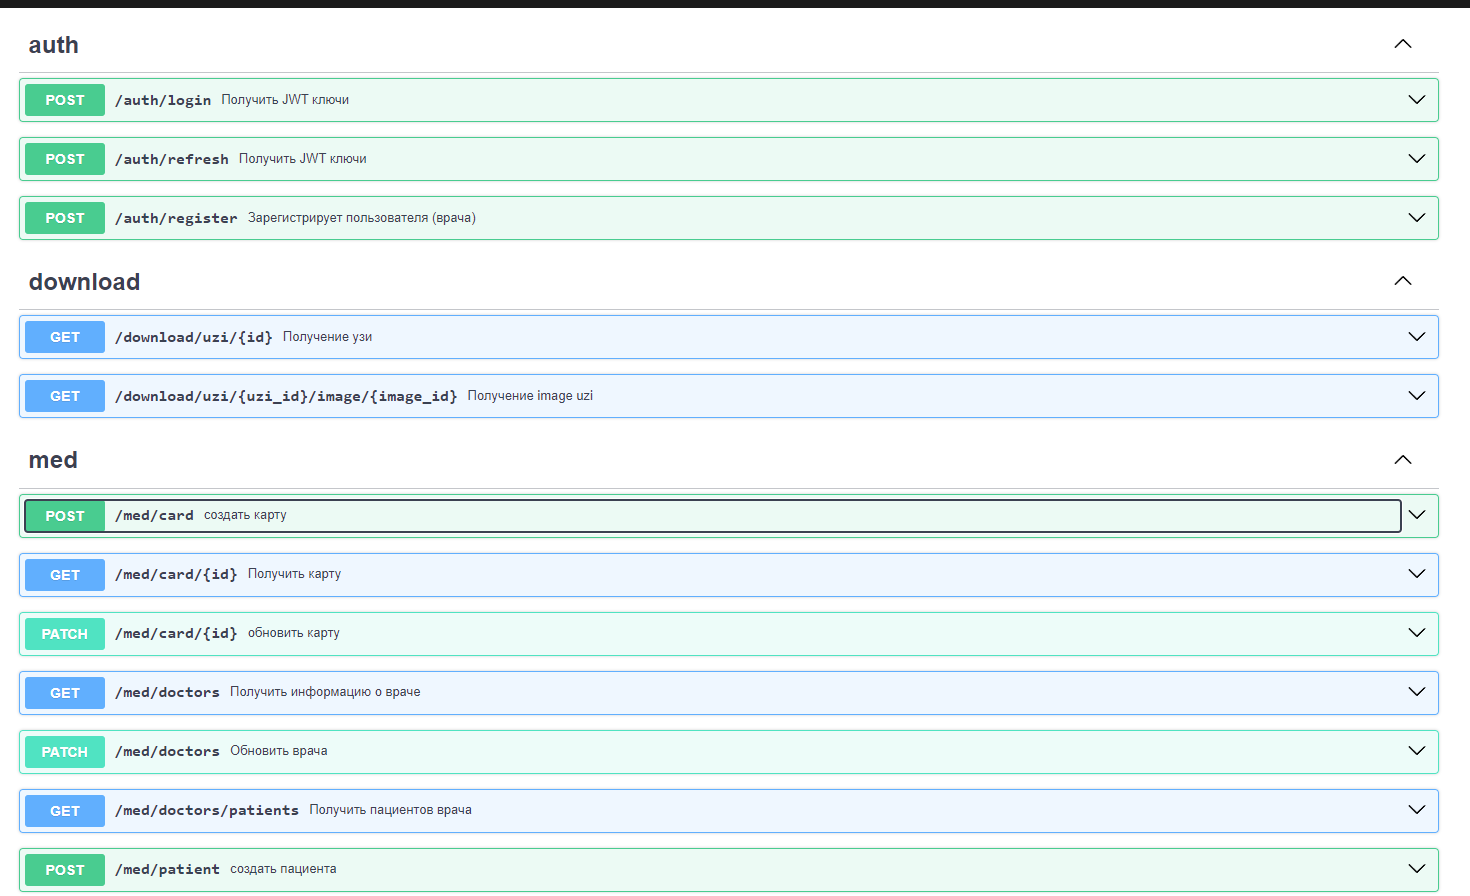
\includegraphics[width=.9\columnwidth]{./img/swagger/sw1.png}%
	\end{center}
	\label{pic:auth_model}%
\end{figure}
\begin{figure}[H]%
	\begin{center}
		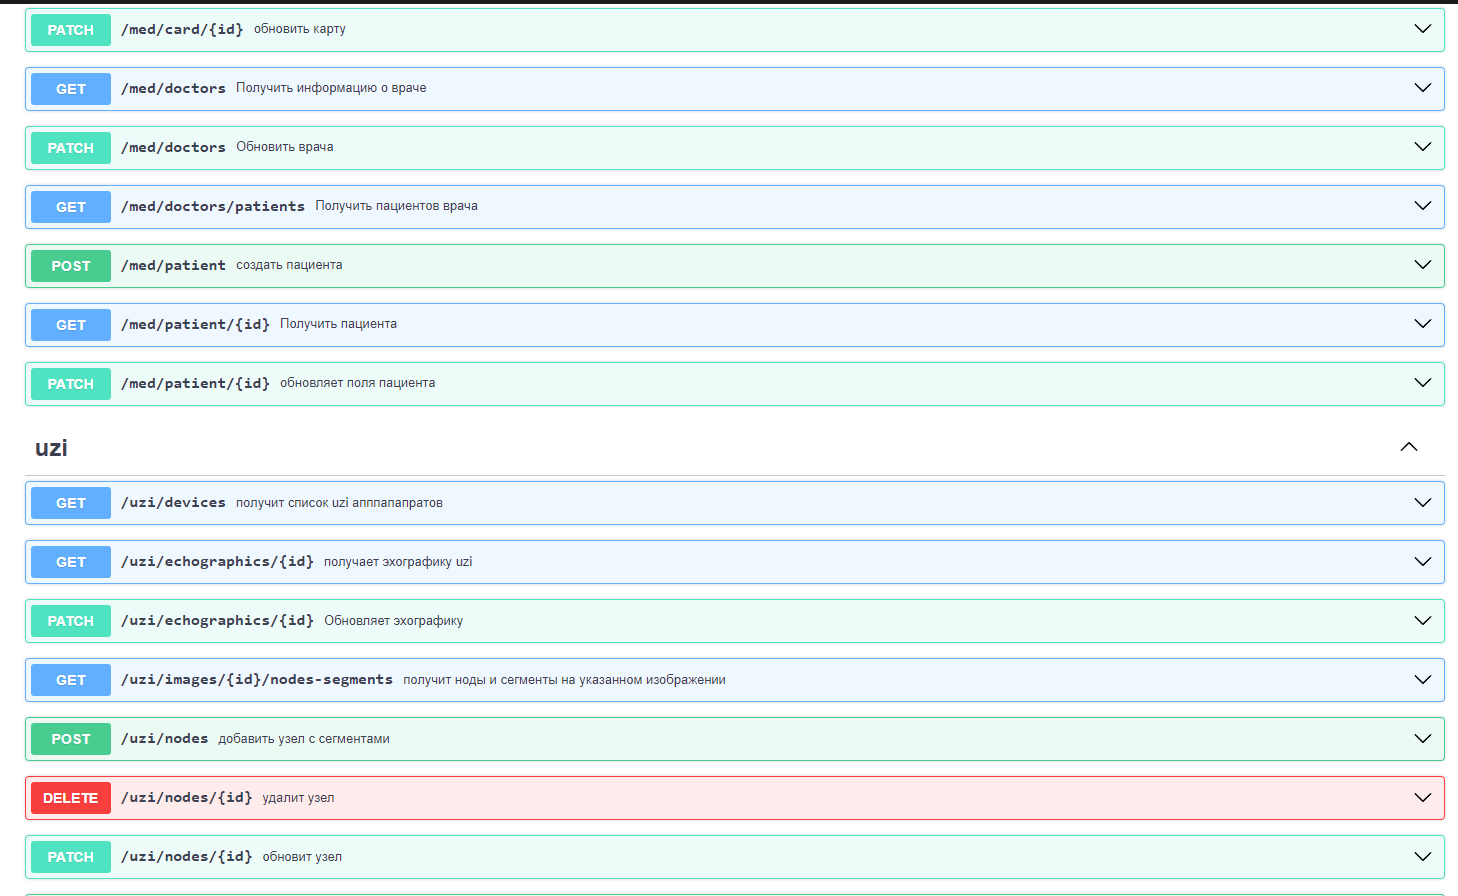
\includegraphics[width=.9\columnwidth]{./img/swagger/sw2.png}%
	\end{center}
	\label{pic:auth_model}%
\end{figure}
\begin{figure}[H]%
	\begin{center}
		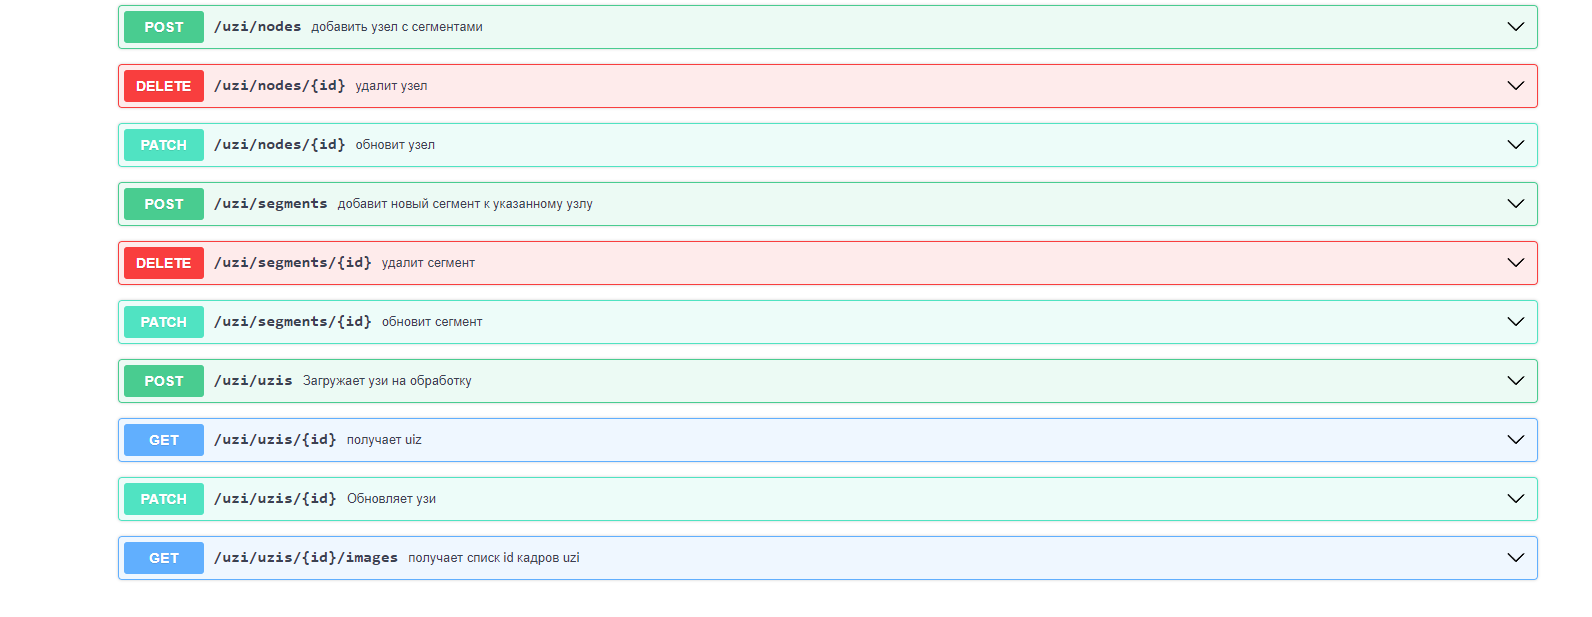
\includegraphics[width=.9\columnwidth]{./img/swagger/sw3.png}%
	\end{center}
	\label{pic:auth_model}%
\end{figure}


%%% Local Variables:
%%% TeX-engine: xetex
%%% eval: (setq-local TeX-master (concat "../" (seq-find (-cut string-match ".*-3-pz\.tex$" <>) (directory-files ".."))))
%%% End:


\label{end_of_document}

% \input{chapters/thesis-template-appendix3.tex}

%\end{appendices}

%%% Local Variables:
%%% TeX-engine: xetex
%%% eval: (setq-local TeX-master (concat "../" (seq-find (-cut string-match ".*-3-pz\.tex$" <>) (directory-files ".."))))
%%% End:
